\documentclass[a4paper, 12pt]{book}
\usepackage[english]{babel}
%\usepackage{mathpazo}
% page layout
\usepackage[left=20mm, right=20mm, top=25mm]{geometry}
\geometry{a4paper}

% appendices
\usepackage[toc,page]{appendix}

% images
\usepackage{graphicx}

% colored headings
\usepackage{xcolor}

% equation numbering
\usepackage{amsmath}
\makeatletter
\def\tagform@#1{\maketag@@@{\ignorespaces\sffamily(#1)\unskip\@@italiccorr}}
\makeatother

% bookmarks
\usepackage{bookmark}

% dedication
\newenvironment{dedication}
{\clearpage             % new page
 \thispagestyle{empty}  % no header and footer
 \vspace*{\stretch{1}}  % top space
 %\itshape               % italics text
 \raggedleft            % flush to the right margin
}
{\par                   % end paragraph
 \vspace{\stretch{3}}   % bottom space (3x top space)
 \clearpage             % finish page
}

% sectioning
\usepackage{titlesec}

% titleformat{name}
% {title style}
% {number style}
% {space between number and title}
% {before-title code}

\titleformat{\part}[display]
  {\normalfont \sffamily \bfseries \centering}
  {\color{red!70!black} \Large \partname \, \thepart}
  {10pt} % vertical spacing
  {\Huge}

\titleformat{\chapter}[display]
  {\normalfont \sffamily \bfseries}
  {\color{red!70!black} \large \chaptertitlename \, \thechapter}
  {1pt}
  {\titlerule[1pt] \vspace{7pt} \Huge}

\titleformat{\section}
  {\normalfont \sffamily \Large}
  {\color{blue!70!black} §\bfseries\thesection}
  {10pt}
  {\bfseries}

\titleformat{\subsection}
  {\normalfont \sffamily \large}
  {\color{blue!70!black} §\bfseries\thesubsection}
  {10pt}
  {\bfseries}

\titleformat{\subsubsection}
  {\normalfont \sffamily}
  {\color{red!70!black} §\bfseries\thesubsubsection}
  {10pt}
  {\bfseries}

\renewcommand{\appendixtocname}{\sffamily Appendices}
\renewcommand{\appendixpagename}{\sffamily \Huge \bfseries Appendices}

% custom table of contents
\usepackage{tocloft}

\renewcommand{\cfttoctitlefont}{\sffamily \Huge \bfseries} % title font
% part
\renewcommand{\cftpartfont}{\sffamily \large \bfseries}
\renewcommand{\cftpartpagefont}{\sffamily \large \bfseries}
\renewcommand{\cftpartpresnum}{\sffamily \color{red!70!black}}
% chapter
\renewcommand{\cftchapfont}{\sffamily \bfseries}
\renewcommand{\cftchappagefont}{\sffamily \bfseries}
\renewcommand{\cftchappresnum}{\sffamily \color{red!70!black}}
% section
\renewcommand{\cftsecfont}{\sffamily}
\renewcommand{\cftsecpagefont}{\sffamily}
\renewcommand{\cftsecpresnum}{\sffamily \color{blue!70!black}}
% subsection
\renewcommand{\cftsubsecfont}{\sffamily}
\renewcommand{\cftsubsecpagefont}{\sffamily}
\renewcommand{\cftsubsecpresnum}{\sffamily \color{blue!70!black}}

% unnumbered chapter
\titleformat{name = \chapter, numberless}[block]
  {\centering \sffamily \bfseries \Large}
  {}
  {0pt}
  {}

% headers and foooters
\usepackage{fancyhdr}
\setlength{\headheight}{15pt}

% part name
\let\Oldpart\part
\newcommand{\parttitle}{}
\renewcommand{\part}[1]{\Oldpart{#1}\renewcommand{\parttitle}{#1}}

% no random page numbers
\fancypagestyle{plain}{%
  \fancyhf{} % clear all header and footer fields
  \renewcommand{\headrulewidth}{0pt}
  \renewcommand{\footrulewidth}{0pt}
}

% custom headers and footers
\renewcommand{\chaptermark}[1]{\markboth{#1}{#1}}
\pagestyle{fancy}
\fancyhead{}
\fancyfoot{}

\fancypagestyle{body}{%
  \fancyhead[LE,RO]{\sffamily\thepage}%
  \fancyhead[LO]{\sffamily \color{blue!70!black}\chaptername\ \thechapter\color{black} :\ \leftmark}%
  \fancyhead[RE]{\sffamily \color{blue!70!black}\partname\ \thepart\color{black} :\ \parttitle}%
}

% special header for Introduction
\fancypagestyle{introd}{%
  \fancyhead[LE,RO]{\sffamily \thepage}%
  \fancyhead[RE,LO]{\sffamily \leftmark}%
}

% special header for Contents
\fancypagestyle{contents}{%
  \fancyhead[LE,RO]{\sffamily \thepage}%
  \fancyhead[RE,LO]{\sffamily }%
}

% special header for Appendix
\fancypagestyle{append}{%
  \fancyhead[LE,RO]{\sffamily \thepage}%
  \fancyhead[LO]{\sffamily \color{blue!70!black}\appendixname\ \thechapter \color{black}:\ \leftmark}%
  \fancyhead[RE]{\sffamily Appendices}%
}

% special header for Bibliography
\fancypagestyle{biblio}{%
  \fancyhead[LE,RO]{\sffamily \thepage}%
  \fancyhead[RE,LO]{\sffamily Bibliography}%
}

% no blank pages
\let\cleardoublepage\clearpage
% removes indentation
\setlength{\parindent}{0pt}
% add subsubsection numbering
\setcounter{secnumdepth}{3}

% math
\usepackage{amsmath}
\usepackage{amssymb}
\usepackage{amsfonts}
\usepackage{amsthm}
\usepackage{mathtools}
\usepackage{mathrsfs}
%\usepackage{tensor}

% physics
\usepackage{braket}

% chemistry
\usepackage{chemformula}

% footnotes
\usepackage{footnote}

% bold text

\newcommand{\bctxt}[1]{\textcolor{blue!70!black}{\textbf{#1}}}

\newcommand{\bcdef}[1]{\textcolor{green!35!black}{\textbf{#1}}}

\newcommand{\bcth}[1]{\textcolor{red!35!black}{\textbf{#1}}}

\newcommand{\bclemma}[1]{\textcolor{blue!35!black}{\textbf{#1}}}

\newcommand{\bcprop}[1]{\textcolor{cyan!35!black}{\textbf{#1}}}

\newcommand{\bcex}[1]{\textcolor{yellow!35!black}{\textbf{#1}}}

% fancy environments
\usepackage[many]{tcolorbox}
\BeforeBeginEnvironment{tcolorbox}{\savenotes}
\AfterEndEnvironment{tcolorbox}{\spewnotes}

\tcbuselibrary{theorems}

\NewTcbTheorem[number within=section]{definition}{Definition}{%
  enhanced,%
  breakable,%
  colback = green!5,%
  colframe = green!5,%
  coltitle = green!35!black,%
  fonttitle = \sffamily\bfseries,%
  sharp corners,%
  boxrule = 0pt,%
  detach title,%
  before upper = {\tcbtitle\\[4pt]},%
  left = 5pt,%
  right = 5pt,%
  top = 5pt,%
  bottom = 5pt,%
  separator sign none,%
  description delimiters parenthesis,%
  description font = \mdseries%
}{def}

\newtcbtheorem[number within=section]{theorem}{Theorem}{%
  enhanced,%
  breakable,%
  colback = red!5,%
  colframe = red!5,%
  coltitle = red!35!black,%
  fonttitle = \sffamily\bfseries,%
  sharp corners,%
  boxrule = 0pt,%
  detach title,%
  before upper = {\tcbtitle\\[4pt]},%
  left = 5pt,%
  right = 5pt,%
  top = 5pt,%
  bottom = 5pt,%
  separator sign none,%
  description delimiters parenthesis,%
  description font = \mdseries%
}{th}

\newtcbtheorem[number within=tcb@cnt@theorem]{corollary}{Corollary}{%
  enhanced,%
  breakable,%
  colback = red!5,%
  colframe = red!5,%
  coltitle = red!35!black,%
  fonttitle = \sffamily\bfseries,%
  sharp corners,%
  boxrule = 0pt,%
  detach title,%
  before upper = {\tcbtitle\\[4pt]},%
  left = 5pt,%
  right = 5pt,%
  top = 5pt,%
  bottom = 5pt,%
  separator sign none,%
  description delimiters parenthesis,%
  description font = \mdseries%
}{cor}

\newtcbtheorem[number within=section]{lemma}{Lemma}{%
  enhanced,%
  breakable,%
  colback = blue!5,%
  colframe = blue!5,%
  coltitle = blue!35!black,%
  fonttitle = \sffamily\bfseries,%
  sharp corners,%
  boxrule = 0pt,%
  detach title,%
  before upper = {\tcbtitle\\[4pt]},%
  left = 5pt,%
  right = 5pt,%
  top = 5pt,%
  bottom = 5pt,%
  separator sign none,%
  description delimiters parenthesis,%
  description font = \mdseries%
}{lemma}

\newtcbtheorem[number within=lemma]{lemcorollary}{Corollary}{%
  enhanced,%
  breakable,%
  colback = blue!5,%
  colframe = blue!5,%
  coltitle = blue!35!black,%
  fonttitle = \sffamily\bfseries,%
  sharp corners,%
  boxrule = 0pt,%
  detach title,%
  before upper = {\tcbtitle\\[4pt]},%
  left = 5pt,%
  right = 5pt,%
  top = 5pt,%
  bottom = 5pt,%
  separator sign none,%
  description delimiters parenthesis,%
  description font = \mdseries%
}{cor}

\newtcbtheorem[number within=section]{proposition}{Proposition}{%
  enhanced,%
  breakable,%
  colback = cyan!5,%
  colframe = cyan!5,%
  coltitle = cyan!35!black,%
  fonttitle = \sffamily\bfseries,%
  sharp corners,%
  boxrule = 0pt,%
  detach title,%
  before upper = {\tcbtitle\\[4pt]},%
  left = 5pt,%
  right = 5pt,%
  top = 5pt,%
  bottom = 5pt,%
  separator sign none,%
  description delimiters parenthesis,%
  description font = \mdseries%
}{prop}

\newtcbtheorem[number within=proposition]{propcorollary}{Corollary}{%
  enhanced,%
  breakable,%
  colback = cyan!5,%
  colframe = cyan!5,%
  coltitle = cyan!35!black,%
  fonttitle = \sffamily\bfseries,%
  sharp corners,%
  boxrule = 0pt,%
  detach title,%
  before upper = {\tcbtitle\\[4pt]},%
  left = 5pt,%
  right = 5pt,%
  top = 5pt,%
  bottom = 5pt,%
  separator sign none,%
  description delimiters parenthesis,%
  description font = \mdseries%
}{cor}

\newtcbtheorem[number within=section]{example}{Example}{%
  enhanced,%
  breakable,%
  colback = yellow!10,%
  colframe = yellow!5,%
  coltitle = yellow!35!black,%
  fonttitle = \sffamily\bfseries,%
  sharp corners,%
  boxrule = 0pt,%
  detach title,%
  before upper = {\tcbtitle\\[4pt]},%
  left = 5pt,%
  right = 5pt,%
  top = 5pt,%
  bottom = 5pt,%
  separator sign none,%
  description delimiters parenthesis,%
  description font = \mdseries%
}{ex}

\newtcolorbox{proofbox}{%
  enhanced,%
  breakable,%
  colback = black!5,%
  colframe = black!5,%
  sharp corners,%
  boxrule = 0pt,%
  left = 5pt,%
  right = 5pt,%
  top = 5pt,%
  bottom = 5pt,%
  borderline west = {1pt}{0pt}{black!70},%
}

% custom references
\newcommand{\eref}[1]{\textsf{Eq.\,\ref{#1}}}
\newcommand{\eeref}[2]{\textsf{Eq.\,\ref{#1}-\ref{#2}}}
\newcommand{\dref}[1]{\textsf{Def.\,\ref{#1}}}
\newcommand{\ddref}[2]{\textsf{Def.\,\ref{#1}-\ref{#2}}}
\newcommand{\tref}[1]{\textsf{Th.\,\ref{#1}}}
\newcommand{\pref}[1]{\textsf{Prop.\,\ref{#1}}}
\newcommand{\lref}[1]{\textsf{Lemma\,\ref{#1}}}
\newcommand{\exref}[1]{\textsf{Ex.\,\ref{#1}}}

\newcommand{\secref}[1]{\textcolor{red!70!black}{\textsf{§\ref{#1}}}}

% hyper-references
\usepackage{hyperref}
\hypersetup{
  colorlinks = true,
  urlcolor = cyan,
  % linkcolor defined directly in \toc environment
  citecolor = green!70!black,
}

\newcommand{\toc}{%
  \hypersetup{linkcolor = black}%
  \tableofcontents%
  \hypersetup{linkcolor = red!70!black}%
}

% extended integral symbols
\usepackage{esint}

% text
\newcommand{\virgolette}[1]{``\text{#1}"}
\newcommand{\tildetext}{\raise.17ex\hbox{$\scriptstyle\mathtt{\sim}$}}

% greek
\newcommand{\Chi}{\text{X}}

% custom math symbols
\newcommand{\abs}[1]{\left\lvert#1\right\rvert}
\newcommand{\norm}[1]{\left\lVert#1\right\rVert}
\newcommand{\sgn}[1]{\mathrm{sgn}\,#1}
\newcommand{\pa}{\partial}
\newcommand{\na}{\nabla}
\newcommand{\tens}[1]{\mathrm{#1}}
\newcommand{\defeq}{\mathrel{\vcenter{\baselineskip0.5ex \lineskiplimit0pt
                     \hbox{\scriptsize.}\hbox{\scriptsize.}}}%
                     =}
\newcommand{\eqdef}{=%
                     \mathrel{\vcenter{\baselineskip0.5ex \lineskiplimit0pt
                     \hbox{\scriptsize.}\hbox{\scriptsize.}}}}
\newcommand{\ve}[1]{\mathbf{#1}}
\newcommand{\hilb}{\mathscr{H}}
\newcommand{\fock}{\mathscr{F}}
\DeclareMathOperator{\diag}{diag}
\newcommand{\sqg}{\sqrt{\tens{g}}}
\newcommand{\sqgm}{\sqrt{-\tens{g}}}
\newcommand{\cm}{\mathcal{C}^{\infty}(\mathcal{M})}
\DeclareMathOperator{\lspan}{span}
\newcommand{\xm}{\mathfrak{X}(\mathcal{M})}
\DeclareMathOperator{\id}{id}
\newcommand{\ld}{\mathcal{L}}
\newcommand{\lm}[1]{\Lambda^{#1}(\mathcal{M})}
\newcommand{\hrm}[1]{\mathrm{Harm}^{#1}(\mathcal{M})}
\DeclareMathOperator{\ran}{ran}
\DeclareMathOperator{\tr}{tr}
\DeclareMathOperator{\Tr}{Tr}
\DeclareMathOperator{\End}{End}
\DeclareMathOperator{\im}{Im}
\newcommand{\dd}{\mathrm{d}}
\newcommand{\bs}[1]{\boldsymbol{#1}}
\newcommand{\dg}{^\dagger}
\DeclareMathOperator{\Aut}{Aut}
\DeclareMathOperator{\ad}{ad}
\DeclareMathOperator{\Ad}{Ad}
\newcommand{\lag}{\mathcal{L}}
\newcommand{\ham}{\mathcal{H}}
\newcommand{\act}{\mathcal{S}}
\newcommand{\normord}{\mathfrak{N}}
\newcommand{\tempord}{\mathfrak{T}}
\newcommand{\parity}{\mathcal{P}}
\newcommand{\chargec}{\mathcal{C}}
\newcommand{\timer}{\mathcal{T}}
\newcommand{\covder}{D}
\newcommand{\mat}{\mathcal{M}}
\newcommand{\smo}{\mathcal{O}}
\newcommand{\msb}{\overline{\text{MS}}}

\newcommand{\grad}{\boldsymbol{\nabla}}
\newcommand{\dive}{\boldsymbol{\nabla}\cdot}
\newcommand{\rot}{\boldsymbol{\nabla}\times}
\newcommand{\lap}{\triangle}

% small \overleftrightarrow
\makeatletter
\newcommand{\overleftrightsmallarrow}{\mathpalette{\overarrowsmall@\leftrightarrowfill@}}
\newcommand{\overrightsmallarrow}{\mathpalette{\overarrowsmall@\rightarrowfill@}}
\newcommand{\overleftsmallarrow}{\mathpalette{\overarrowsmall@\leftarrowfill@}}
\newcommand{\overarrowsmall@}[3]{%
  \vbox{%
    \ialign{%
      ##\crcr
      #1{\smaller@style{#2}}\crcr
      \noalign{\nointerlineskip}%
      $\m@th\hfil#2#3\hfil$\crcr
    }%
  }%
}
\def\smaller@style#1{%
  \ifx#1\displaystyle\scriptstyle\else
    \ifx#1\textstyle\scriptstyle\else
      \scriptscriptstyle
    \fi
  \fi
}
\makeatother
\newcommand{\smlra}[1]{\overleftrightsmallarrow{#1}}
\newcommand{\smla}[1]{\overleftsmallarrow{#1}}
\newcommand{\smra}[1]{\overrightsmallarrow{#1}}

% functions
\DeclareMathOperator{\sech}{sech}
\DeclareMathOperator{\Exp}{Exp}

% number sets
\newcommand{\N}{\mathbb{N}}
\newcommand{\Z}{\mathbb{Z}}
\newcommand{\Q}{\mathbb{Q}}
\newcommand{\R}{\mathbb{R}}
\newcommand{\C}{\mathbb{C}}
\newcommand{\K}{\mathbb{K}}

% groups
\newcommand{\Ot}{\mathrm{O}(3)}
\newcommand{\SOt}{\mathrm{SO}(3)}
\newcommand{\On}[1]{\mathrm{O}(#1)}
\newcommand{\SOn}[1]{\mathrm{SO}(#1)}
\newcommand{\Un}[1]{\mathrm{U}(#1)}
\newcommand{\SUn}[1]{\mathrm{SU}(#1)}
\newcommand{\GL}[1]{\mathrm{GL}(#1)}
\newcommand{\SL}[1]{\mathrm{SL}(#1)}

% units of measure
\newcommand{\m}{\,\mathrm{m}}
\newcommand{\ang}{\,\mathrm{\AA}}
\newcommand{\fm}{\,\mathrm{fm}}

\newcommand{\barn}{\,\mathrm{barn}}

\newcommand{\cels}{\,^{\circ}\mathrm{C}}

\newcommand{\ev}{\,\mathrm{eV}}
\newcommand{\kev}{\,\mathrm{keV}}
\newcommand{\mev}{\,\mathrm{MeV}}
\newcommand{\gev}{\,\mathrm{GeV}}
\newcommand{\tev}{\,\mathrm{TeV}}

% particles
\newcommand{\g}{\mathrm{g}}
\newcommand{\w}{\mathrm{W}}
\newcommand{\z}{\mathrm{Z}}

% custom title page
\newcommand{\customtitlepage}[7]{%
  \begin{titlepage}
    \centering
    % department logo at the top of the page
    
\includegraphics[width=0.75\textwidth]{imgs/unimi.jpg}\\
    \vspace{1cm} % ddjust the vertical space as needed
    {\large Bachelor's Degree in #1 \par} % degree title
    \vspace{1cm}
    %\hrule % horizontal line
    \vspace{1cm} % adjust the vertical space as needed
    {\large \sffamily \textbf{#2} \par} % thesis title (bold)
    \vspace{9cm} % adjust the vertical space as needed
    
    \begin{minipage}[H]{\textwidth}
      \small Supervisor: \\
      \normalsize #3 \\
      \vspace{1cm}
    \end{minipage}
    \begin{minipage}[t]{\textwidth}
      \raggedleft
      \small Student: \\
      \normalsize #4\\ % student name
      \normalsize Matr.: #5 % student number
    \end{minipage}

    % academic year section at the bottom of the page
    \vspace{\fill}
    {\normalsize Academic Year #6 \par}
    
  \end{titlepage}
}

\usepackage[font=small]{caption}
\newcommand{\um}{\mathfrak{m}}

\usepackage{overarrows}
\usepackage{slashed}
\usepackage{simpler-wick}
\usepackage{amsmath,amssymb}
\usepackage{bbold}

\usepackage{tikz}
\usepackage[compat=1.1.0]{tikz-feynman}
\usetikzlibrary{arrows.meta}


% bibliography

\usepackage{csquotes}
\usepackage[
backend = biber,
style = numeric-comp,
sorting = ynt
]{biblatex}
\addbibresource{bibl.bib}

\renewbibmacro{in:}{}

\AtEveryBibitem{%
	\clearfield{publisher}%
	\clearfield{month}%
	\clearfield{numpages}%
	\clearfield{issue}%
	\clearfield{isbn}%
}

\DeclareFieldFormat[book,article]{journaltitle}{#1}
\DeclareFieldFormat[book,article]{volume}{\mkbibbold{#1}}


\title{Thesis}
\author{Lucrezia Bioni}

\begin{document}

\frontmatter

\customtitlepage{Physics}{Next-to-Leading Order QCD Corrections to Scattering Processes Using $\theta$-Parameters in the Nested Soft-Collinear Subtraction Scheme}{Prof. Raoul Horst Röntsch}{Lucrezia Bioni}{13655A}{2024--2025}
\clearpage

\chapter*{Abstract}
\selectlanguage{english}
Perturbative Quantum Chromodynamics (QCD) corrections are essential for achieving high-precision theoretical predictions in particle physics, which makes them fundamental for interpreting data from modern particle accelerators, such as the Large Hadron Collider (LHC) at CERN. As experimental precision increases, theoretical predictions must also attain a level of accuracy that allows for meaningful comparisons with data. This requires extending perturbative calculations beyond the leading order (LO) to include next-to-leading order (NLO) and higher-order corrections in the strong coupling constant $\alpha_s$. These corrections account for crucial physical effects, such as real parton emissions and virtual loop contributions. \\
A significant challenge in calculating these higher-order corrections arises from the presence of infrared (IR) singularities, which occur when partons become soft or collinear. Although the sum of all contributions to a cross-section is finite, due to the cancellation of divergences between real emissions and virtual loops, each individual term is divergent. To manage these divergences and obtain finite, numerically stable results, it is necessary to introduce subtraction schemes that regularize the singularities locally in the phase space. \\
Over the past few decades, a variety of subtraction schemes have been developed for this purpose. Among them, the Nested Soft-Collinear (NSC) Subtraction Scheme has gained particular prominence due to its conceptual clarity, modular structure, and consistent extensibility from NLO to next-to-next-to-leading order (NNLO). The NSC scheme achieves a local cancellation of infrared singularities by factorizing soft and collinear limits in a nested manner. Furthermore, its modular nature allows the subtraction terms for complex processes to be built from a limited set of basic components, making it well-suited for implementation in automated Monte Carlo frameworks. \\
The aim of this thesis is to extend the NSC Subtraction Scheme by introducing a set of continuous parameters, called $\theta$-parameters, which systematically restrict the subtraction procedure to the singular, unresolved regions of phase space where soft and collinear singularities occur. Specifically, the parameter $\theta_s$ limits the energy of unresolved partons in the soft limit, while $\theta_i$ controls their angular separation in the collinear limit. The central motivation for this development is to improve numerical stability and efficiency in Monte Carlo integrations, particularly for multi-leg processes where redundant phase-space coverage can significantly slow down convergence. \\
The implementation and analytical study in this thesis demonstrate that introducing $\theta$-parameters preserves the theoretical consistency and modular nature of the NSC scheme. These parameters modify only the soft and collinear (real) contributions, while leaving the virtual corrections and those from PDF renormalization unchanged. Specifically, they appear in the $I_{\mathrm{S}}(\epsilon)$ and $I_{\mathrm{C}}(\epsilon)$ operators, which are part of the soft and collinear counterterms for the infrared-divergent scattering amplitudes. Crucially, the $\theta$-parameters do not compromise the cancellation of the infrared $1/\epsilon^2$ and $1/\epsilon$ poles when all contributions are summed. The coefficient of the $1/\epsilon^2$ pole in $I_{\mathrm{S}}(\epsilon)$ is independent of any parameter, and, while the coefficients of the $1/\epsilon$ poles in $I_{\mathrm{S}}(\epsilon)$ and $I_{\mathrm{C}}(\epsilon)$ depend on $\theta_s$, this dependence cancels out in their sum. This confirms that the modified NSC scheme yields the same physical cross-sections as the standard one. \\
Therefore, the study presented in this thesis contributes to the ongoing effort to improve the efficiency and reliability of higher-order QCD computations. Such improvements are fundamental to continue testing the Standard Model and searching for new Physics beyond its confines.


\newpage

\newgeometry{left=25mm, right=25mm, top=25mm, bottom=25mm}
\pagestyle{contents}

\toc

\restoregeometry
\pagestyle{body}

\mainmatter


\chapter{Introduction}

\section{The Standard Model}


As Aristotle stated, women and men began to philosophize due to wonder. From antiquity, a profound sense of astonishment towards the natural world has driven humans to investigate phenomenological reality. This drive is so profound and innate in humanity that – starting with the first philosophers, called ``Pre-Socratics"  or ``natural philosophers" – it led them to inquire into the nature of the ``archè" ($\acute{\alpha}\rho\chi\acute{\eta}$), the primordial principle and fundamental constituent underlying all of nature. This enduring pursuit of fundamental knowledge evolved through the centuries and, in the last one, culminated in the experimental discovery of a multitude of subatomic particles. Their proliferation was such that it prompted the noted physicist Enrico Fermi to remark: ``If I could remember the names of all these particles, I'd be a botanist". This apparent complexity, however, has been successfully resolved through the development of a robust theoretical framework that classifies these particles and describes their interactions via gauge theories: the Standard Model (SM). \\
The SM is formulated within the mathematical framework of Quantum Field Theory (QFT), which unifies the principles of Quantum Mechanics and Special Relativity to describe phenomena at high energies, or equivalently, subatomic scales. Its predictions have been rigorously tested and confirmed by experiments, most notably with the discovery of the Higgs boson in 2012.  Despite its success, there are significant efforts to discover Physics beyond the SM. This is driven not only by the natural attempt at falsification that should be applied to every scientific theory, but also by several phenomena that the model cannot explain. These include the existence of dark matter and dark energy, the observed matter-antimatter asymmetry, and the origin of neutrino masses \cite{Campbell:2017}. \\

\section{Collider physics}
One of the principal methods of research in high-energy physics is collider physics \cite{ellis}. Using colliders, it is possible to artificially accelerate particles and to reach extremely high center-of-mass energy. Operating at the energy frontier is crucial: higher-energy collisions enable events with greater momentum transfer and energy deposition. These events are essential because concentrating significant energy within a tiny volume allows us to excite new, heavy elementary particles from the vacuum, and study their properties. Experiments at the energy frontier are conducted at the Large Hadron Collider (LHC) at CERN: in a 27-kilometer ring, proton beams collide at a center-of-mass energy of approximately 13.6 TeV. Although these energy scales have allowed us to study the known fundamental interactions – with the exception of gravity – in great detail, they have not been sufficient for the discovery of new particles.  Since increasing the energy of the colliding particles is not feasible with existing technology, the focus of collider experiments in the next decade will shift towards higher experimental precision. This precision is crucial for refining our understanding of the Standard Model (SM), especially the properties of the Higgs boson: in fact, it is the agent of electroweak (EW) symmetry breaking, which is a fundamental component of the theory. Moreover, precision measurements serve as a powerful probe for new physics, which may reveal itself as subtle deviations from SM predictions in processes involving only known particles.  However, testing the Standard Model with experimental results necessitates reliable theoretical predictions for hadron collider processes.

\section{QCD and hard scattering processes}
A theoretical description of hadron collisions is complicated primarily by our limited knowledge of the strong force, which binds the elementary constituents of hadrons. Strong interactions are described by Quantum Chromodynamics (QCD), a non-Abelian gauge theory based on the SU(3) symmetry group. The QCD Lagrangian is not analytically solvable, making it extremely difficult to understand proton dynamics from first principles. A way to overcome these obstacles becomes manifest when we consider how hadrons collide at high energies \cite{Asteriadis2020}. Typically, they undergo either elastic scattering or diffractive dissociation: in the first case, they collide but remain intact; in the second, they disintegrate into a small number of hadrons. However, on rare occasions, a more interesting phenomenon can occur: the elementary partons that compose the hadrons can interact and exchange a large amount of momentum ($\sim 100 \,\text{GeV}$). This is the case in so-called ``hard scattering processes," which are central to probing the electroweak scale, the Higgs boson, and potential new physics. Their importance is directly related to a key feature of the strong force: asymptotic freedom. The essence of this property is the weakening of the colour force at short distances \cite{ellis}. In this high-energy regime, the interacting partons can be approximated as being nearly free, which permits a perturbative description of the strong interaction. The strength of these interactions is governed by the coupling constant $\alpha_{\text{S}}$. Due to asymptotic freedom, $\alpha_{\text{S}}$ is on the order of $0.1$ at energies relevant for contemporary colliders\footnote{This value is energy-dependent; $\alpha_{\text{S}}\sim0.1$ is typical at energies around 100 GeV.}. This makes the strong force about ten times stronger than the electromagnetic interaction (whose coupling constant is $\alpha\sim1/137$), yet sufficiently small to allow for the application of well-defined perturbative approximation methods.

\section{Hadronic cross-section and factorization theorem}
A framework for describing these short-distance hard scattering processes is provided by the collinear factorization theorem \cite{Collins:1987pm}. Within this framework, colliding hadrons are treated as beams of partons, each carrying a certain fraction of the hadron's total momentum. The probability of finding a parton with a specific energy fraction is encoded in the Parton Distribution Functions (PDFs). These functions are universal, meaning they are independent of the specific scattering process being studied. Consequently, PDFs can be measured in one set of experiments and then used to make predictions for many others \cite{Melnikov2018}. The short-distance interaction of partons produces final states composed of Standard Model particles, such as leptons, gauge bosons, and additional QCD partons. The final-state partons, which are the direct products of the perturbative calculation, cannot be observed directly due to confinement\footnote{Quark confinement is the phenomenon that prevents quarks and gluons from propagating as free particles over macroscopic distances.}. Instead, they evolve into collimated sprays of hadrons \cite{Salam:2010nqg}. We interpret these partons as the seeds of hadronic jets and define the resulting sprays as jets themselves. At high energies, the properties of these jets are largely determined by the perturbative dynamics of their initiating parton and are only mildly affected by non-perturbative QCD effects. \\
The asymptotic freedom of QCD is what enables a perturbative description of the strong interaction. However, it is crucial to recognize that the precise mechanism allowing us to decouple the motion of partons from the proton's dynamics is the separation of energy scales involved. Interactions in the Standard Model typically probe energy scales on the order of $Q \sim 100  \, \text{GeV} - 1 \, \text{TeV}$, while the characteristic energy scale of hadronic structure and confinement is significantly lower, $\Lambda_{\text{QCD}} \sim 100 \, \text{MeV}$. \\
The production cross section for final states involving QCD jets and other Standard Model particles in hard hadronic collisions is thus given by
\begin{equation}
    \text{d}\sigma = \sum_{a, b} \int_0^1 \text{d}x_1 \text{d}x_2 \, f_{a}(x_1, \mu_\text{F}) \, f_{b}(x_2,\mu_\text{F}) \, \text{d}\hat \sigma_{a,b}(x_1,x_2,\mu_\text{F},\mu_\text{R};\mathcal{O}) \, \left(1+ \mathcal{O}\left(\frac{\Lambda_{\text{QCD}}}{Q} \right)^n \right), \qquad n\geq1
    \label{fact-theor}
\end{equation}
where $f_{a,b}$ are the parton distribution functions mentioned above; $a, b \in \{g, d/\bar{d}, u/\bar{u}, s/\bar{s}, c/\bar{c}, b/\bar{b} \}$  represent the types of partons (gluons or quarks) inside the two colliding hadrons; $x_1, x_2$ are respectively the momentum fractions carried by partons $a$ and $b$; and $\mathcal{O}$ is an infrared-finite observable. \\
The non-perturbative corrections in Eq. \ref{fact-theor} are suppressed by powers of the ratio $\Lambda_{\text{QCD}}/Q$: in this case, $Q$ represents the hard scale of the process, typically identified as the lowest transverse momentum ($p_T$) cut applied to final-state partons. For a typical cut of $Q \sim 20\ \text{GeV}$, this ratio is of order $10^{-2}$. The exact power $n$ of this suppression is process-dependent, and not always immediately evident, though for many applications the leading power is $n = 2$. This implies that the theoretical uncertainty from factorizing non-perturbative physics is of order $\mathcal{O}(10^{-4})$. Even when the leading power is only $n = 1$, the non-perturbative effects would be at the percent level ($\sim 10^{-2}$). This is comparable in size to the Next-to-Next-to-Leading Order (NNLO) QCD corrections for many processes. Therefore, a precise description of a process requires the inclusion of at least NNLO perturbative corrections before the inherent uncertainty from power corrections becomes significant.\\
This formalism establishes a clear distinction between the short-distance perturbative process and the long-distance non-perturbative physics. The boundary between these two regimes is defined by the factorization scale ($\mu_\text{F}$). Processes with a momentum transfer $Q > \mu_\text{F}$ are treated as the hard scatter of point-like partons, calculable within perturbation theory. Physics at scales $Q < \mu_\text{F}$, which describes how the partons are bound within the proton, is incorporated into the non-perturbative Parton Distribution Functions (PDFs). \\
The other scale present in the factorized cross-section in Eq. \ref{fact-theor} is the renormalization scale ($\mu_\text{R}$). Its necessity arises because the calculation of partonic interactions in QCD using Feynman diagrams often results in ultraviolet (UV) divergences. These infinities do not indicate a fundamental error in the theory, but suggest a distinction between the bare parameters in the Lagrangian and physically observable quantities. The process of renormalization allows us to absorb these divergences into a redefinition of the Lagrangian's parameters, providing finite expressions for measurable quantities. The consequence of this procedure is that the coupling constant becomes a function of the energy scale, a phenomenon known as ``running" \cite{ellis}. The renormalization scale $\mu_\text{R}$ is the energy at which the coupling constant is defined, thereby encapsulating the quantum corrections of the theory. \\
Throughout this thesis, we set $\mu_\text{F} = \mu_\text{R} = \mu$. While a physical prediction must be independent of these arbitrary scales, cross-sections calculated within a fixed-order perturbative expansion exhibit a dependence on both the renormalization and factorization scales. Therefore, varying the scales around a central value and observing how the prediction changes provides a standard method for estimating the uncertainty associated with the truncation of the perturbative series. \\

\begin{figure}[!ht]
	\centering
	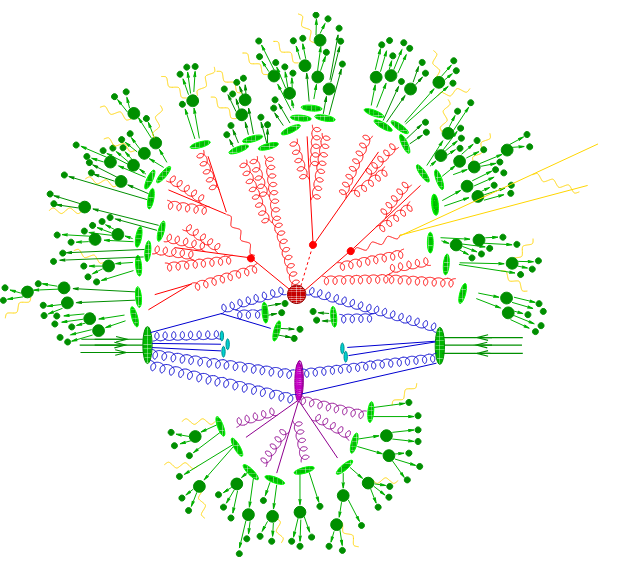
\includegraphics[width=0.7\textwidth]{imgs/hadron-collision.png}
	\caption{Sktetch of an hard hadron-hadron collision at a collider like the LHC. The central red blob represents the hard interaction, a high-energy collision between two partons, calculable using perturbative QCD. The incoming and outgoing partons emit initial-state (blue) and final-state (red) radiation, producing many secondary particles. Softer underlying event activity (purple) arises from additional partonic interactions within the protons. A key feature is the hierarchy of energy scales: the hard process occurs at high energies ($Q>\Lambda_{\text{QCD}}$), while subsequent radiation and hadronization (green) take place at progressively lower scales, eventually transitioning to non-perturbative physics around $\Lambda_{\text{QCD}}$. Figure from \cite{Hoeche:2014}.}
	\label{hadron-collision}
\end{figure}

Referring to Eq. \ref{fact-theor}, we can state that only the left-hand side represents a physically measurable quantity. The right-hand side, in contrast, consists of unobservable components: the parton distribution functions (PDFs), which are extracted from experimental data, and the partonic cross-section $\mathrm{d}\hat{\sigma}_{a,b}$, which is calculable within perturbation theory. It is therefore essential to understand how this latter quantity is computed.


\section{Partonic cross-section}
We consider the inclusive\footnote{The inclusive cross-section counts every collision event that creates a specific particle, whether it appears alone, with jets, or with any other additional radiation. It gives the total production rate, ignoring the details of what else is produced alongside it.} production of $N$ jets at a hadron collider, together with a color-neutral system $X$
\begin{equation}
    pp \rightarrow X + N \, \mathrm{jets}  \, .
\end{equation}
As discussed above, we can use asymptotic freedom of QCD to expand the partonic cros section $\mathrm{d}\hat{\sigma}_{a,b}$ in Eq. \ref{fact-theor} in powers of the strong and the electroweak coupling constants, $\alpha_{\text{S}}$ and $\alpha$,
\begin{equation}
    \text{d} \hat{\sigma}_{a,b} = \text{d} \hat{\sigma}_{a,b}^{(0,0)} + \alpha_s \text{d} \hat{\sigma}_{a,b}^{(1,0)} + \alpha_s^2 \text{d} \hat{\sigma}_{a,b}^{(2,0)} + \alpha_s^3 \text{d} \hat{\sigma}_{a,b}^{(3,0)} + \alpha \text{d} \hat{\sigma}_{a,b}^{(0,1)} + \alpha \alpha_s \text{d} \hat{\sigma}_{a,b}^{(1,1)} + \dots .
\end{equation}
Due to the different values of the coupling constants, at the same order they have a different impact on the final result: at NLO, QCD corrections account for approximately $10\%$, while EW account for $1\%$; at NNLO, QCD corrections account for $1\%$. Throughout this thesis, we will focus on the calculation of NLO QCD corrections. \\
The first term in this expansion $\text{d} \hat{\sigma}_{a,b}^{(0,0)} \equiv \text{d} \hat{\sigma}_{a,b}^{\text{LO}}$ is called Leading Order (LO), and it is defined as \cite{Devoto:2025jql}
\begin{equation}
    2s_{a,b}\text{d} \hat{\sigma}_{a,b}^{\text{LO}} = \mathcal{N} \int \mathrm{d}\Phi (2\pi)^4 \mathrm{dLips}_X \delta^{(4)}(p_\mathcal{H_f}+p_X-p_a-p_b) \left|\mathcal{M}_0(p_a,p_b;p_{\mathcal{H}_f},p_X) \right|^2 \mathcal{O}(p_\mathcal{H},p_X).
    \label{leading-order}
\end{equation}
With $\mathcal{H}_f$, we denote the list of final-state resolved particles, and $p_{\mathcal{H}_f}$ is their momentum, while $p_X$ denotes the momentum of the color-singlet in the hard process. $\mathcal{N}$ is a normalization factor: it takes into account color and spin averages as well as symmetry factors. With $s_{a,b}$, we express the partonic center-of-mass energy squared: $s=(p_a+p_b)^2=2 p_a\cdot p_b$, considering massless partons. The matrix element for the considered process is denoted by $\mathcal{M}_0$, and $\mathcal{O}$ represents an infrared-safe observable that ensures the final state contains at least $N$ resolved jets. This latter feature is crucial because infrared dynamics are non-perturbative and, consequently, cannot be described by an expansion in $\alpha_\mathrm{s}$. Finally, $\mathrm{dLips}_X$ is the Lorentz-invariant phase space for the colorless particle $X$, including the momentum-conserving delta function, and $\mathrm{d}\Phi$ is the Lorentz-invariant phase space for the final-state particles.
\begin{equation}
    \mathrm{d}\Phi= \prod_{i \in \mathcal{H}_f} [\mathrm{d}p_i], \qquad [\mathrm{d}p_i]=\frac{\mathrm{d}^3p_i}{(2\pi)^32E_i},
\end{equation}
where $[\mathrm{d}p_i]$ is the phase-space element of a final-state parton $i$. Moreover, in Eq. \ref{leading-order}, summation over spins and colors of final-state partons, and averaging over spins and colors of initial-state partons are assumed.  \\
For notational compactness, we introduce the function $F^{ab}_{\mathrm{LM}}$, defined as in Section 2 of \cite{Devoto:2023rpv}
\begin{equation}
    F^{ab}_{\mathrm{LM}} = \mathrm{dLips}_X |\mathcal{M}_0|^2 \, \mathcal{O}.
    \label{flm}
\end{equation}
We denote the integration over the final-state phase space of Eq. \ref{flm} with the angular brackets $\langle\dots\rangle$, and obtain exactly Eq. \ref{leading-order}
\begin{equation}
    2s_{a,b} \, \text{d} \hat{\sigma}_{a,b}^{\text{LO}} = \langle F^{ab}_{\mathrm{LM}}[\dots] \rangle.
\end{equation} \\
At Leading Order (LO), calculations are performed directly. The tree-level matrix elements can be computed easily using helicity techniques and colour-subamplitude decompositions \cite{Altarelli:1977zs}, and are then integrated, either numerically or analytically. \\
The strong coupling constant in hard scattering processes is small enough to allow for a perturbative description, but not enough to make higher-order corrections entirely negligible. Therefore, in order to claim high precision, we also need to compute QCD corrections. According to the factorization theorem, the computed partonic cross-section should be insensitive to long-distance effects, which are absorbed into the parton distribution functions. The QCD corrections instead account for short-distance, high-energy effects at higher orders in the coupling constant. The NLO correction $\text{d} \hat{\sigma}_{a,b}^{(1,0)} \equiv \text{d} \hat{\sigma}_{a,b}^{\mathrm{NLO}} $ to a partonic cross section consists of three terms: the one-loop (virtual) contribution, the real emission contribution, and the contribution related to parton distribution functions


\begin{equation}
    \mathrm{d} \hat{\sigma}_{a,b}^{\mathrm{NLO}} = \mathrm{d} \hat{\sigma}_{a,b}^{\mathrm{V}} + \mathrm{d} \hat{\sigma}_{a,b}^{\mathrm{R}} + \mathrm{d} \hat{\sigma}_{a,b}^{\mathrm{pdf}}.
\end{equation} 

The last term, $\mathrm{d} \hat{\sigma}_{a,b}^{\mathrm{pdf}}$, is generated by the renormalization of the PDFs at LO, and its expression is known \cite{Catani:1996vz}. The other terms, $\mathrm{d} \hat{\sigma}_{a,b}^{\mathrm{V}}$ and $\mathrm{d} \hat{\sigma}_{a,b}^{\mathrm{R}}$, are related to either the emission of an additional leg in the Feynman diagram, i.e., an extra parton in the final state (real correction), or to the emission and reabsorption of a parton through a loop (virtual correction).  \par\bigskip
\begin{figure}[!ht]
	\centering
	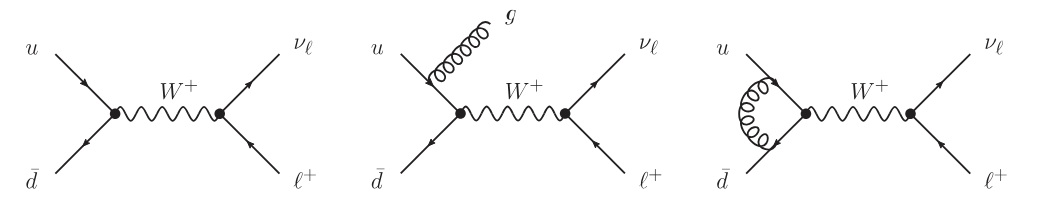
\includegraphics[width=0.9\textwidth]{imgs/real-and-virtual.png}
	\caption{Feynman diagrams for W boson production at hadron colliders. The diagram on the left corresponds to the leading-order (LO) calculation of the total cross-section. The diagrams shown in the middle and on the right represent the real and virtual corrections, respectively, which together constitute the next-to-leading-order (NLO) contributions to the total cross-section. Figure from \cite{Campbell:2017}}.
	\label{hadron-collision}
\end{figure}
It is important to emphasize that while the concepts of ``real" and ``virtual" radiation are physically well-defined, their separate contributions to the partonic cross-section, $\mathrm{d}\hat{\sigma}_{a,b}$, are not physically observable. The division into real and virtual terms is therefore a computational tool, introduced to organize the calculation and manage the various contributions more effectively. \\ The treatment of these terms is non-trivial, as they exhibit divergences in specific energy regimes. The virtual contributions, for instance, contain ultraviolet (UV) singularities. These are removed through the process of renormalization\footnote{Throughout this thesis, we work with UV-renormalized matrix elements.}, a procedure that ensures physical observables, when expressed in terms of appropriately defined renormalized parameters, become insensitive to the high-energy UV region. \\ Furthermore, the low-momentum (soft) and small-angle (collinear) kinematic regions produce singularities in both the real and virtual contributions. These infrared (IR) singularities are not independent: the real and virtual corrections are fundamentally linked by their infrared behavior. The divergence of scattering amplitudes in the soft or collinear limit means these kinematic configurations must be carefully handled to obtain meaningful results. Consequently, a precise procedure for removing these divergences is of the highest importance for calculating finite cross-sections.

\section{Infrared poles and their cancellation}
In order to deal with IR divergences, it is convenient to employ dimensional regularization \cite{THOOFT1973455}. This technique involves the analytical continuation of momentum space from $4$ to $d=4-2\epsilon$ dimensions, where $\epsilon \in \mathbb{C}$ and $\mathrm{Re}(\epsilon)<0$. In this framework, divergences appear as poles in $1/\epsilon$ in the complex dimensional plane. \\
The virtual corrections $\mathrm{d} \hat{\sigma}_{a,b}^{\mathrm{V}}$ contain explicit infrared and collinear poles, which are independent of the details of the hard matrix element \cite{Catani:1996vz}. In contrast, the real emission contribution $\mathrm{d} \hat{\sigma}_{a,b}^{\mathrm{R}}$ contains kinematic singularities that only become explicit $1/\epsilon$ poles upon integration over the phase space of the additional final-state parton. However, we must avoid a naive integration over the entire radiation phase space, as it would render the cross section inclusive rather than differential, discarding all information on the kinematics of the radiated parton. This information is often crucial since jet properties provide essential data for defining experimental signatures. \\
QCD amplitudes for real emission processes become singular in kinematic limits where the gluon becomes soft (low energy) or any parton (quark, antiquark, gluon) is emitted collinearly to another parton. In these limits, the propagator of the emitted particle approaches its on-shell condition, leading to divergent behavior. To show this, consider a diagram that describes an emission of a gluon ($\um$) off an external incoming quark ($i$) line 
\begin{equation*}
  \begin{tikzpicture}[baseline = (r.base)]
    \begin{feynman}[inline = (r.base)]
      \vertex (a);
      \vertex[right = 2.5cm of a, dot] (b) {};
      \vertex[right = 2.5cm of b, circle, draw, fill=lightgray,  minimum size = 1.2cm] (c) {};

      \vertex[above = 1cm of b] (d);
      \vertex[right = 1.5cm of d] (e);

      \vertex[below = 0.25cm of b] (r);

      \diagram* {
	    (a) -- [fermion, momentum' = \(p_i\)] (b),
	    (b) -- [fermion, momentum' = \(p_i - p_\um\)] (c),

	    (b) -- [gluon, momentum = \(p_\um\)] (e),
        };
    \end{feynman}
  \end{tikzpicture}
  \quad \sim \quad
  \frac{1}{(p_i - p_\um)^2} = \frac{1}{2 E_i E_\um \left( 1 - \cos \theta_{i \um} \right)} \quad
  \xrightarrow[E_\um, \theta_{i \um} \to 0 ]{} \quad \infty \,.
\end{equation*}
For massless partons ($|\mathbf{p}_i|=E_i, \, |\mathbf{p}_i|^2=0$), the amplitude exhibits a clear divergence in both the soft and collinear limits, that is when $E_\um$ or $\theta_{i \um} \to 0$.\\
It is important to consider the origin of these infinities. The presence of divergences is, in fact, a manifestation of long-distance effects: they signal that non-perturbative contributions are entering our perturbative calculation. This could be a problem, as we lack methods to treat non-perturbative QCD effects from first principles \cite{Melnikov2018}. Fortunately, once the $1/\epsilon$ poles are extracted from both the virtual and real corrections, their sum is guaranteed to be free of infrared divergences due to the Bloch-Nordsieck \cite{PhysRev.52.54} and Kinoshita-Lee-Nauenberg theorems. Therefore, perturbative QCD corrections remain insensitive to the details of infrared physics. \\
However, achieving the cancellation of the $1/\epsilon$ poles by simply summing the real and virtual corrections is not straightforward. This complication arises because the virtual corrections are defined in an $n$-particle phase space, whereas the real corrections inhabit an ($n+1$)-particle phase space. We might think that this problem could be avoided by integrating over the phase space. However, this approach would only yield a total cross-section, not a differential one, as stated above. This mismatch in the dimensionality of the integration domains, combined with the need to extract the implicit $1/\epsilon$ poles from the real-emission contributions, without performing the full integration, is precisely why dedicated subtraction schemes are required. \\
Over time, various methods have been developed to perform fully differential QCD computations for hadron collider processes, both at NLO and NNLO. Among the existing methods, in this thesis we will focus on the Nested Soft-Collinear (NSC) Subtraction Scheme \cite{Caola:2017dug}, which will be detailed in Chapter \ref{NSC-SS}. The numerical stability and computational efficiency of this method can, however, be further improved. A step forward in this direction will be presented in Chapter \ref{NSC-SS-parameters}; this represents the original contribution of this thesis. 


\clearpage

\chapter{NLO QCD corrections in the NSC Subtraction Scheme}
\label{NSC-SS}
The singular limits of NLO QCD amplitudes, as well as the methods for using them to compute NLO QCD cross sections, are well established \cite{Frixione:1995ms,Catani:1996vz}. Furthermore, all the singular limits of QCD amplitudes necessary for calculating NNLO QCD corrections have been known for approximately two decades \cite{Catani:1996vz}. However, it took significant time to determine how to use these NNLO limits to construct a valid subtraction method for NNLO computations due to the presence of overlapping singularities at this orde. Among the numerous proposed methods, the Nested Soft-Collinear Subtraction Scheme (NSC SS), introduced in \cite{Caola:2017dug}, is particularly attractive, for reasons that will become clear throughout the following discussion. \\
This chapter provides an overview of the main results achieved. Since the objective of this thesis is to implement parameters that allow for greater control over the integrated phase-space region, and since these parameters appear only in the real corrections, we will focus exclusively on the latter. Moreover, the IR-divergent parts of the virtual corrections can be isolated using Catani's representation of renormalized one-loop scattering amplitudes \cite{Catani:1998bh}. Although these methods have been implemented up to NNLO \cite{Caola:1902, Caola:1907, Asteriadis:1910, Devoto:2023rpv, Devoto:2025kin}, this thesis will focus on the NLO case, as its relative simplicity offers a clearer understanding of how to implement the parameters.

\section{Properties of Soft and Collinear partons}
\label{properties}
A subtraction scheme necessitates the isolation of singularities in the real corrections without integrating over the momenta of any of the final-state particles, in order to keep the kinematics of all the final-state particles intact. There are two key insights that allow us to overcome this obstacle. The first one is related to the behaviour of NLO QCD amplitudes at soft and collinear limits. \\For a generic QCD amplitude $\mathcal{M}$ involving $n$ partons with four-momenta $p_1, p_2, \dots, p_n$ and an additional soft gluon with vanishing four-momentum $p_\um$, the squared amplitude factorizes into (i) the squared amplitude for the hard process without the gluon and (ii) an eikonal factor that depends only on the color charges and momenta of the hard partons and the momentum of the soft gluon ($p_\um$) \cite{Catani:1999ss}
\begin{equation}
    \lim_{E_\um \rightarrow 0}|\mathcal{M}(p_1, p_2, \dots, p_n; p_\um)|^2= - 4\pi \alpha_s \mu^{2\epsilon} \sum_{i,j=1}^n \mathcal{S}_{ij}(p_\um) \vec{T}_i \cdot \vec{T_j} |\mathcal{M}_0(p_1, p_2, \dots, p_n)|^2,
    \label{ampl-soft}
\end{equation}
where the \emph{general eikonal factor} is
\begin{equation}
    \mathcal{S}_{ij}(p_\um) = \frac{p_i \cdot p_j}{(p_i \cdot p_\um)(p_j \cdot p_\um)}  \,, 
    %\sim \frac{1}{E_\um^2}
    \label{eikonal}
\end{equation}
and the square of the color charges are $\vec{T}_i^2= C_F$ if $i$ is a quark or an anti-quark, and $\vec{T}_i^2= C_A$ if $i$ is a gluon. \\

We now consider the limit where a gluon is emitted parallel to a quark. In this limit, the amplitude-squared factorizes into (i) a \emph{splitting function}, which describes the probability for the quark to radiate the gluon collinearly at a given energy, and (ii) the squared hard amplitude, which now depends on the resulting quark momentum after the emission. More generally, if a parton $[i\um]$ emits a parton $i$ and a parton $\um$, the following factorization formula holds
\begin{equation}
    \lim_{\theta_{i \um \rightarrow 0}}|\mathcal{M}(p_1, \dots, p_n; p_\um)|^2 \sim P_{f_{[i\um]}f_i} (z) |\mathcal{M}_0(p_1, \dots , p_i + p_\um, \dots, p_n)|^2  \,.
    %\sim \frac{1}{(p_i-p_\um)^2} \sim (1-\cos(\theta_{i\um}))^{-1}\sim \theta_{i\um}^{-2}.
    \label{ampl-coll}
\end{equation}
The variable $z$ is a ratio of energies of the collinear partons. This variable, as well as rules for constructing the parton $[i\um]$ from partons $i$ and $\um$, will be discussed in Section \ref{section-coll-soft}. \\

The unresolved parton $\um$ could also be a quark or an antiquark. However, the emission of a soft quark leads to a convergent integral; consequently, no divergences are associated with soft quark or antiquark emissions. Divergences do arise in the collinear limit, but, as in the gluon case, the amplitude factorizes into a hard process involving a parton with rescaled momentum and a corresponding splitting function. \\
Equation \ref{ampl-soft} shows that the dependence on $p_\um$ lies only in the eikonal function, while $\mathcal{M}_0$ is independent of $p_\um$. Instead, Equation \ref{ampl-coll} shows that the dependence on the unresolved momentum is absorbed into the rescaled momentum of parton $i$ within the hard matrix element $\mathcal{M}_0$, while the singular behavior is captured by the splitting function. These remarks will be fundamental to construct properly a subtraction method. \\
The second important insight is that, in singular kinematic regions, real emissions are always unresolved, meaning they lack a distinct experimental signature. Consequently, we can safely integrate over the singular regions of their phase space without losing any physically observable information, a procedure we will carry out in Sections \ref{section-soft-limit} and \ref{section-coll-soft}. 

\section{Why a subtraction method}
Let us first present the core idea of the subtraction formalism. We consider the integral
\begin{equation}
    I = \int_0^1 \mathrm{d}x \, \frac{1}{x^{1+\epsilon}} F(x),
\end{equation}
where $F(x)$ is an arbitrary function regular at $x=0$. The integrand diverges at the lower limit, and this singularity is regulated by the parameter $\epsilon$, which ultimately produces a $1/\epsilon$ pole upon integration. We want to isolate this pole analytically, and define the integral in such a way that the limit $\epsilon \to 0$ can be taken safely. To achieve this, we write $F(x)=[F(x)-F(0)]+F(0)$
\begin{equation}
    I = \int _0^1 \mathrm{d}x \, \frac{1}{x^{1+\epsilon}} [F(x)-F(0)]+F(0)\int_0^1 \mathrm{d}x \, \frac{1}{x^{1+\epsilon}},
\end{equation}
and, performing the integration in the second term, we get
\begin{equation}
    I = \int_0^1 \frac{\mathrm{d}x}{x}[F(x)-F(0)] - \frac{1}{\epsilon}F(0) + \mathcal{O}(\epsilon).
    \label{extraction-poles}
\end{equation}
This equation demonstrates that we have successfully isolated the $1/\epsilon$ pole in $I$ and regulated the integrand. As a result, the $\epsilon \to 0$ limit can now be taken safely, leaving an integral that is regular at $x=0$ and can be evaluated numerically.\\
Let us apply this idea to the case of real emission contributions in NLO calculations. Suppose that we have a function $\mathcal{S}$ that reproduces the leading singular behaviour of $F^{ab}_{\mathrm{LM}}$ (defined in Eq. \ref{flm}) in all soft and collinear limits, and that can be integrated in the $d$-dimensional phase space of the unresolved parton $\um$. We can then write the real-emission cross section as
\begin{equation}
    2s_{a,b} \mathrm{d} \hat{\sigma}_{a,b}^{\mathrm{R}} = \int [\mathrm{d}p_{\um}] F^{ab}_{\mathrm{LM}} = \int [\mathrm{d}p_{\um}] (F^{ab}_{\mathrm{LM}} - \mathcal{S}) + \int [\mathrm{d}p_{\um}] \mathcal{S}
    \label{subtraction-flm}
\end{equation}
where $[\mathrm{d}p_{\um}]$ is the $d$-dimensional phase-space measure for the emitted gluon, now also incorporating the theta function to enforce energy conservation
\begin{equation}
    [\mathrm{d}p_{\um}] = \frac{\mathrm{d}^{d-1}p_\um}{(2 \pi)^{d-1}2E_\um} \theta(E_{\mathrm{max}}-E_\um),
    \label{measure}
\end{equation}
and $E_{\mathrm{max}}$ is an arbitrary energy scale that must be at least as large as the maximum energy allowed by the momentum-conserving $\delta$-functions in Eq. \ref{leading-order}.\\
On the right-hand side of Eq. \ref{subtraction-flm}, the first term is integrable in four-dimensional phase space, since the leading singular behaviour of $F^{ab}_{\mathrm{LM}}$ is removed by the subtraction term $\mathcal{S}$. As this integration is performed numerically using Monte Carlo (MC) methods, it is clear that restricting the integration region to the minimal necessary volume is crucial for improving the efficiency of the computation. We will return to this point in Chapter \ref{NSC-SS-parameters}.\\
The second term involves only the unresolved parton $\um$, making it possible to integrate over its phase space without affecting the jet observables. Furthermore, as showed in Eq. \ref{extraction-poles}, this integration enables the extraction of $1/\epsilon$ poles, which describe the singular behaviour of $\mathcal{S}$ and, consequently, of the amplitude itself. Moreover, it resolves the problem of the dimensional mismatch between the integration domains of the virtual and real corrections. Thus, the cancellation of the poles with those arising from the virtual contributions becomes possible.

\section{Outline of NSC Subtraction Scheme at NLO}
Different subtraction schemes are characterized by different forms for $\mathcal{S}$, or, equivalently, $F(0)$. The FKS subtraction scheme, which constitutes the basis for the NSC method, constructs $\mathcal{S}$ directly from the soft and collinear limits. The efficacy of this approach becomes clear if we consider the behaviour of the amplitudes in these limits, as detailed in Section \ref{properties}: in both the soft and collinear cases, the amplitude squared factorizes into a  lower-multiplicity function $F^{ab}_{\mathrm{LM}}$, and a singular term, whose integration over the phase space of parton $\um$ gives the explicit pole. Therefore, we introduce two operators that perform soft and collinear projections
\begin{equation}
    S_i A = \lim_{E_i \to 0} A \, , \qquad C_{ij}A = \lim_{\rho_{ij}\to 0}A \, ,
    \label{projections}
\end{equation}
where $\rho_{ij}= 1 - \vec{n}_i \cdot \vec{n}_j = 1 - \cos{\theta_{ij}}$, with $\vec{n}_i$ a unit vector that describes the direction of the momentum of the $i$-th particle in ($d-1$)-dimensional space, and $\theta_{ij}$ the angle between partons $i$ and $j$. These operators apply to all terms that follow them. \\
Thus, we identify $\mathcal{S}$ as the action of the soft and/or collinear operators on $F^{ab}_{\mathrm{LM}}$. We also note that these operators are defined to capture the leading asymptotic behaviour of the product of the matrix element squared, the observable, and the phase space – namely, the definition of $F^{ab}_{\mathrm{LM}}$ in Eq. \ref{flm}. Thus, if this quantity is integrable, the operator acts as an annihilator (e.g., $S_q = S_{\bar{q}}=0$). \\
The singularities are isolated and extracted sequentially in a nested manner: first, the soft singularities are removed, followed by the collinear and soft-collinear ones, using an identity operator constructed as follows:
\begin{equation}
    \mathbb{1} = S_\um + \sum_{i \in \mathcal{H}} \bar{ S}_\um C_{i\um} + \sum_{i \in \mathcal{H}} \bar{S}_\um \bar{C}_{i \um} \omega^{\um i} \, ,
    \label{identity-soft-coll}
\end{equation}
where $\bar{ S}_\um= \mathbb{1} - S_\um$, $\bar{ C}_\um= \mathbb{1} - C_\um$, $\mathcal{H} = \mathcal{H}_f \cup \{a,b\}$, and $\omega^{\um i}$ are partition functions that  allow for treating one collinear singularity at a time by splitting the phase space. The partition functions satisfy the following equations
\begin{equation}
    \sum_{i \in \mathcal{H}} \omega^{\um i} = 1 \, , \qquad C_{k\um}\omega^{\um i} = \delta_{ki} \,.
\end{equation}
It is also convenient to partition the phase space in such a way that some partons are classified as ``hard” and thus cannot give rise to infrared singularities. For this purpose, we define so-called ``damping factors” (see Appendix \ref{partition-damping}), which can be used to construct a partition of unity
\begin{equation}
  \sum_{i \in \mathcal{H}_f} \Delta^{(i)}=1 \, .
\end{equation}
The soft and collinear operators acting on the damping factors lead to the following results
\begin{equation}
S_\um \Delta^{(\um)} = 1, \quad C_{a\um} \Delta^{(\um)} = 1, \quad C_{i\um} \Delta^{(\um)} = \frac{E_\um}{E_i+ E_\um} =z_{\um,i},
\end{equation}
for $a = 1,2$ and $i > 3$. The damping factor $\Delta^{(i)}$ acts as an annihilator, vanishing when any parton other than $i$ becomes unresolved. This allows us to unambiguously identify parton $i$ as being potentially unresolved. \\

We now apply the identity in Eq. \ref{identity-soft-coll} to the real-emission contribution $F_{\mathrm{LM}}(\um)$, which gives
\begin{equation}
  \langle \Delta^{(\um)}F_{\mathrm{LM}}(\um) \rangle = \langle S_{(\um)}F_{\mathrm{LM}}(\um) \rangle + \sum_{i=1}^{N_p} \langle \bar{S}_{(\um)}C_{i\um} \Delta^{(\um)} F_{\mathrm{LM}}(\um) \rangle + \langle \bar{S}_{(\um)} \bar{C}_{i\um} \Delta^{(\um)} \omega^{\um i} F_{\mathrm{LM}}(\um) \rangle \, ,
  \label{identity-flm}
\end{equation}
where the final term on the right-hand side is completely finite and can be integrated in four dimensions. It is important to emphasize the convention used for symmetry factors, which follows the same approach as in Ref. \cite{Devoto:2025kin}. Specifically, we define symmetry factors based only on the number  of \emph{resolved} partons, that is, all partons except for the one labeled $\um$.  To clarify this convention, let us consider a general example that will be discussed in more detail in Chapter \ref{NSC-SS-parameters}: the process $a_g + b_q \to X + (N_g+1)g + q$, where $X$ is a color singlet. In this case, the function $F_{\mathrm{LM}}(\um)$ contains symmetry  factors that account for the fact that there are $N_g+1$ ways to choose an unresolved gluon, but 
only one way to choose an unresolved quark. Therefore, we can decompose it as
\begin{equation}
  F_{\mathrm{LM}}(\um) = F_{\mathrm{LM}}^g(\um_g) +F_{\mathrm{LM}}^q(\um_q) \, ,
\end{equation}
where
\begin{equation}
  \begin{aligned}
    & F_{\mathrm{LM}}^g(\um_g) = \frac{1}{N_g!}  F_{\mathrm{LM}}^{ab} \left(\{g\}_{N_g}, \{q\}_1 | \um_g \right) \, , \\
    & F_{\mathrm{LM}}^q(\um_q) = \frac{1}{(N_g+1)!}  F_{\mathrm{LM}}^{ab} \left(\{g\}_{N_g+1}| \um_q \right) \, .
  \end{aligned}
\end{equation}
We note that the symmetry factors multiplying the various $F_{\mathrm{LM}}$ functions are defined by the number of final-state \emph{resolved} gluons. This means that when a gluon is treated as unresolved, the remaining $N_g$ gluons in $F_{\mathrm{LM}}^g(\um_g)$ are considered resolved, and the symmetry factor becomes $1/N_g!$. Similarly, when a quark is unresolved, all $N_g+1$ 
gluons are treated as resolved, leading to a symmetry factor of $1/(N_g+1)!$. This approach ensures consistent counting of identical particles throughout the calculation.

\section{Modularity of the scheme}
\label{modularity-scheme}
One of the most interesting features of the NSC subtraction scheme is its modular structure: the subtractions for a generic process, no matter how complicated, are built from a relatively small set of basic ingredients. Indeed, the soft contributions are straightforward to compute, while, for the nested-hard-collinear ones, we only need to consider pairs of partons. This leads to three possible cases: both partons are initial state, both are final state, or one is initial and one is final. These three possibilities have been studied in \cite{Caola:1902}, \cite{Caola:1907}, and \cite{Asteriadis:1910}, respectively. Therefore, in order to better understand the workings of the NSC subtraction scheme with all its subtleties, the following sections will present a general treatment, while making explicit reference to specific examples, namely the processes discussed in \cite{Caola:1902}, \cite{Caola:1907}, and \cite{Asteriadis:1910}.
\\
Ref. \cite{Caola:1902} provides the analytic formulas for the production of a generic color-singlet final state $V$ at a hadron collider, i.e., $q_1\bar{q}_2 \to V$ (which we will call $\mathcal{P}_{1}^{\mathrm{LO}}$). A simple example is the Drell-Yan process, illustrated in the following diagram
\begin{equation*}
    \mathcal{P}_{1}^{\mathrm{LO}}: \quad q_1 + \bar{q}_2 \to e^+ + e^- \qquad \qquad
  \begin{tikzpicture}[baseline = (current bounding box.center), thin]
    \begin{feynman}[inline = (r.base)]
      % Definizione di TUTTI i vertici
      \vertex (q);                    % quark in entrata
      \vertex[above right=1.5cm of q, dot] (a) {};  % vertice di annichilazione  
      \vertex[ right=2cm of a] (z);    % vertice bosone Z/gamma
      \vertex[above right=1.5cm of z] (l1); % leptone in uscita
      \vertex[below right=1.5cm of z] (l2); % antileptone in uscita
      \vertex[above left=1.5cm of a] (qbar); % antiquark in entrata
      \vertex[below=0.3cm of a] (c);  % punto di riferimento per baseline
      
      % Diagramma - solo connessioni tra vertici definiti
      \diagram* {
        (qbar) -- [anti fermion, red, edge label'=\(\bar{q}_2\)] (a),
        (q) -- [fermion, red, edge label'=\(q_1\)] (a),
        (a) -- [photon, edge label'=\(\gamma^*/Z\)] (z),
        (z) -- [fermion, edge label'=\(e^+\)] (l1),
        (z) -- [anti fermion, edge label'=\(e^-\)] (l2),
      };
    \end{feynman}
  \end{tikzpicture}
\end{equation*}
The real emission contribution refers to the process $\mathcal{P}_{1}^{\mathrm{NLO}}: q_1\bar{q}_2 \rightarrow V+ g_3$, that, in the case of Drell-Yan, can be represented as
\begin{equation*}
    \mathcal{P}_{1}^{\mathrm{NLO}}: \quad q_1 + \bar{q}_2 \to e^+ + e^- + g_3 \qquad \qquad
  \begin{tikzpicture}[baseline = (current bounding box.center), thin]
    \begin{feynman} [inline = (r.base)]
      % Definizione di TUTTI i vertici
      \vertex (a);                    % quark in entrata
      \vertex[right=1.5cm of a, dot] (b) {};  % vertice di annichilazione  
      \vertex[right=1.5cm of b] (c);
      \vertex[below=1.5cm of a] (d);
      \vertex[right=1.5cm of d, dot] (e) {};
      \vertex[right=1.5 of e] (f);
      \vertex[above right=1.5 of f] (g);
      \vertex[below right=1.5 of f] (h);
      
      % Diagramma - solo connessioni tra vertici definiti
      \diagram* {
        (a) -- [fermion, edge label'= \(q_1\)] (b),
        (b) -- [gluon, edge label' = \(g_3\)] (c),
        (b) -- [fermion] (e),
        (d) -- [anti fermion, edge label'=\(\bar{q}_2\)] (e),
        (e) -- [photon] (f),
        (f) -- [fermion, edge label'=\(e^+\)] (g),
        (f) -- [anti fermion, edge label'=\(e^-\)] (h),
      };
    \end{feynman}
  \end{tikzpicture}
\end{equation*}
Instead, Ref. \cite{Caola:1907} considers the decay of a color-singlet particle $Q$ into quarks and gluons, and, in particular, the process $\mathcal{P}_{2}^{\mathrm{LO}}: Q \to f_i f_j + X$, where $\{f_i,f_j\}$ can be either $\{g,g\}$ or $\{q,\bar{q}\}$. We will focus on the discussion of the decay to a $gg$ final state since its singularity structure is more complex: once the corrections for $Q \to gg$ are understood, the corrections for $Q\to q \bar{q}$ are easily derived. This process, if for instance $Q$ is the Higgs boson, is represented by the following diagram
\begin{equation*}
    \mathcal{P}_{2}^{\mathrm{LO}}: H \to g_1 + g_2 \qquad \qquad
    \begin{tikzpicture}[baseline = (current bounding box.center), thin]
    \begin{feynman} [inline = (r.base)]
      \vertex (a) {\(H\)};                   
      \vertex[right=1.5cm of a, circle, draw, minimum size=1pt, inner sep=0pt,] (b) {\(\times\)};   
      \vertex[above right =1.5cm of b] (c);
      \vertex[below right =1.5cm of b] (d);
      
      \diagram* {
        (a) -- [dashed] (b),
        (b) -- [gluon, red, edge label' = \(g_1\)] (c),
        (b) -- [gluon,red,  edge label' = \(g_2\)] (d),
      };
    \end{feynman}
  \end{tikzpicture}
\end{equation*}
where $\otimes$ denotes the effective local vertex, which encapsulates the top-quark loop contribution. \\NLO QCD contributions come from the following process
\begin{equation*}
  \mathcal{P}_{2}^{\mathrm{NLO}}: H \to g_1 + g_2 + g_3\qquad
  \begin{tikzpicture}[baseline = (current bounding box.center), thin]
    \begin{feynman} [inline = (r.base)]
      % Higgs
      \vertex (H) at (-1.5,0) {\(H\)};
      % Vertice efficace Hgg (⊗)
      \vertex (Heff) at (0,0) [circle, draw, minimum size=10pt, inner sep=0pt] {\(\times\)};
      % Nodo intermedio per il 3-gluon vertex
      \vertex (gvert) at (1,0) [dot] {};
      % gluoni finali
      \vertex (g1) at (2,1.2) {};
      \vertex (g2) at (2,0.0) {};
      \vertex (g3) at (2,-1.2) {};

      % connessioni
      \diagram* {
        (H) -- [dashed] (Heff),
        % due gluoni prodotti direttamente dal vertice efficace
        (Heff) -- [gluon, edge label=\(g_1\)] (g1),
        (Heff) -- [gluon] (gvert),
        % splitting a tre gluoni
        (gvert) -- [gluon, edge label=\(g_2\)] (g2),
        (gvert) -- [gluon, edge label=\(g_3\)] (g3),
      };
    \end{feynman}

  \end{tikzpicture}
\end{equation*}

% deep inelastic scattering commented: this example is not significative to the comprehension of the mechanism

Finally, Ref. \cite{Asteriadis:1910} provides the NLO QCD corrections for the deep-inelastic scattering process of an electron on a proton. At leading order, this receives contributions from both the processes $\mathcal{P}_{3}^{\mathrm{LO}}: q_1 + e^-_2 \to e^-_3 + q_4$ and $\bar{q} + e^- \to e^- + \bar{q}$. However, since these are identical, we will consider only the first one, which is illustrated in the following diagram
\begin{equation*}
    \mathcal{P}_{3}^{\mathrm{LO}}: q_1 + e^-_2 \to e^-_3 + q_4 \qquad \qquad
    \begin{tikzpicture}[baseline = (current bounding box.center), thin]
    \begin{feynman} [inline = (r.base)]
      \vertex (a) {};                   
      \vertex[right=1.5cm of a, dot] (b) {};   
      \vertex[right=1.5cm of b] (c);
      \vertex[below=1.5cm of a] (d);
      \vertex[right=1.5cm of d, dot ] (e) {}; 
      \vertex[right=1.5cm of e] (f);
      
      \diagram* {
        (a) -- [fermion, red, edge label'=\(q_1\)] (b),
        (b) -- [fermion, red, edge label'=\(q_4\)] (c),
        (b) -- [photon] (e),
        (d) -- [fermion, edge label'=\(e^-_2\)] (e),
        (e) -- [fermion, edge label'=\(e^-_3\)] (f),
      };
    \end{feynman}
  \end{tikzpicture}
\end{equation*}
The real emission contribution at NLO refers to the process $\mathcal{P}_{3}^{\mathrm{NLO}}: q_1 + e^-_2 \to e^-_3 + q_4 + g_5$, where the gluon becomes collinear to the incoming or the outcoming quark

\begin{equation*}
\mathcal{P}_{3}^{\mathrm{NLO}}: q_1 + e^-_2 \to e^-_3 + q_4 + g_5 \qquad
\begin{minipage}{0.2\textwidth}
\centering
\begin{tikzpicture}[baseline = (current bounding box.center), thin]
  \begin{feynman}
    \vertex (a) {};    
    \vertex[right=0.75cm of a] (m);               
    \vertex[right=0.75cm of m, dot] (b) {};   
    \vertex[right=1.5cm of b] (c);
    \vertex[below=1.5cm of a] (d);
    \vertex[right=1.5cm of d, dot ] (e) {}; 
    \vertex[right=1.5cm of e] (f);
    \vertex[above=0.75cm of m] (g);

    \diagram* {
      (a) -- [fermion, edge label'=\(q_1\)] (b),
      (m) -- [gluon, edge label'=\(g_5\)] (g),
      (b) -- [fermion, edge label'=\(q_4\)] (c),
      (b) -- [photon] (e),
      (d) -- [fermion, edge label'=\(e^-_2\)] (e),
      (e) -- [fermion, edge label'=\(e^-_3\)] (f),
    };
  \end{feynman}
\end{tikzpicture}
\end{minipage}
\hfill
\begin{minipage}{0.2\textwidth}
\centering
\begin{tikzpicture}[baseline = (current bounding box.center), thin]
  \begin{feynman}
    \vertex (a) {};    
    \vertex[right=0.75cm of b] (m);               
    \vertex[right=1.5cm of a, dot] (b) {};   
    \vertex[right=1.5cm of b] (c);
    \vertex[below=1.5cm of a] (d);
    \vertex[right=1.5cm of d, dot ] (e) {}; 
    \vertex[right=1.5cm of e] (f);
    \vertex[above=0.75cm of m] (g);

    \diagram* {
      (a) -- [fermion, edge label'=\(q_1\)] (b),
      (m) -- [gluon, edge label'=\(g_5\)] (g),
      (b) -- [fermion, edge label'=\(q_4\)] (c),
      (b) -- [photon] (e),
      (d) -- [fermion, edge label'=\(e^-_2\)] (e),
      (e) -- [fermion, edge label'=\(e^-_3\)] (f),
    };
  \end{feynman}
\end{tikzpicture}
\end{minipage}
\end{equation*}

Our goal is to present the explicit expression for the real-emission contributions in a form similar to that of Catani's $I_1(\epsilon)$ function defined in Ref.\cite{Catani:1998bh}, by introducing two operators, $I_{\mathrm{S}}(\epsilon)$ and $I_{\mathrm{C}}(\epsilon)$, which parametrize the poles arising from the soft and collinear limits, respectively. The corrections will then be given by the product of these functions with the leading-order kinematics, so that the sum
\begin{equation}
I_{\mathrm{T}}(\epsilon) = I_{\mathrm{V}}(\epsilon) + I_{\mathrm{S}} (\epsilon)+ I_{\mathrm{C}}(\epsilon) \, ,
\end{equation}
is finite as $\epsilon \to 0$, where $I_{\mathrm{V}}(\epsilon)$ is related to $I_1(\epsilon)$. 

In Section~\ref{section-soft-limit}, we will derive the $I_\mathrm{S}$ operator for a generic process and then demonstrate how to recover the results of Refs.~\cite{Caola:1907} and \cite{Asteriadis:1910} for the two specific processes considered in those references. Subsequently, we will derive the $I_\mathrm{C}$ operator in Section~\ref{section-coll-soft}, where we will also show how it connects to the specific examples presented in Refs.~\cite{Caola:1902} and \cite{Caola:1907}.
  
\section{Soft limit}
\label{section-soft-limit}
Let $\um$ be the index that characterizes the unresolved parton. To obtain the first term on the right-hand side of Eq.~\ref{identity-flm}, it is necessary to integrate over the phase space of the parton $\um$ in Eq.~\ref{ampl-soft}, which represents the result of the soft operator acting on the squared matrix element.Before performing the integration, we note that it is convenient to express the phase-space measure $[\mathrm{d}p_\um]$ from Eq. \ref{measure} in hyperspherical coordinates. For massless partons (where $|p_\um|=E_\um$), this measure becomes
\begin{equation}
  [\mathrm{d}p_\um] = \frac{E_\um^{d-3} \,\mathrm{d}E_\um  \, \mathrm{d}\Omega_{d-1}}{2 (2 \pi)^{d-1}} \, \theta(E_{\mathrm{max}}-E_\um) \, ,
  \label{measure-ps}
\end{equation}
where ${d}\Omega_{d-1}$ is the ($d-1$)-dimensional hyperspherical measure. Using the bare QCD coupling $g_{s,b}^2 = 4\pi\alpha_s$ and considering $N_p$ partons at Leading Order, we obtain
\begin{equation}
  \langle S_\um F_{\mathrm{LM}} (\um) \rangle = \int \mathrm{d}E_\um E_\um^{d-5} \, \theta(E_{\mathrm{max}}-E_\um)  \int \frac{\mathrm{d}\Omega_{d-1}}{2 (2 \pi)^{d-1}} (-g_{s,b}^2) \sum_{(i \neq j)}^{N_p} \frac{\rho_{ij}}{\rho_{im}\rho_{jm}} (\vec{T}_i \cdot \vec{T}_j) F_{\mathrm{LM}} \, ,
\end{equation}
where we do not list all the partons involved in the process as arguments of $F_{\mathrm{LM}}$, but we only 
specify if it depends on the unresolved parton $\um$. Recall that $\rho_{ij} = 1 - \cos\theta_{ij}$, so that the dot product is $p_i \cdot p_j = E_i E_j \rho_{ij}$. We now evaluate the integrals using dimensional regularization in $d=4-2\epsilon$ dimensions. The energy integral yields a simple pole in $\epsilon$
\begin{equation}
  \int_0^{E_{\mathrm{max}}} \frac{\mathrm{d}E_\um}{ E_\um^{1+2\epsilon}} = - \frac{1}{2 \epsilon} E_{\mathrm{max}}^{-2 \epsilon} \, .
\end{equation}
Regarding the angular integral, we utilize a standard result, given for instance in Appendix G.2 of \cite{Asteriadis:1910}
\begin{equation}
  \int \frac{\mathrm{d}\Omega_{d-1}}{2 (2 \pi)^{d-1}} \frac{\rho_{ij}}{\rho_{ik}\rho_{jk} } = - \frac{2^{1-2\epsilon}}{\epsilon} \left[\frac{1}{8 \pi^2} \frac{(4\pi)^{\epsilon}}{\Gamma(1-\epsilon)}  \right]\eta_{ij}^{-\epsilon} K_{ij} \, ,
\end{equation}
with
\begin{equation}
  K_{ij} = \left[ \frac{\Gamma^2(1-\epsilon)}{\Gamma(1-2\epsilon)}\right] \eta_{ij}^{1+\epsilon} \, {}_2F_1(1,1;1-\epsilon; 1-\eta_{ij}) \, ,
  \label{k-function}
\end{equation}
where $\eta_{ij}=\rho_{ij}/2$, and ${}_2F_1$ denotes the Gauss hypergeometric function. Combining these results, we get 
\begin{equation}
   \langle S_\um F_{\mathrm{LM}} (\um) \rangle = - \frac{[\alpha_s]}{\epsilon^2} \left(\frac{2 E_{\mathrm{max}}}{\mu}\right)^{-2\epsilon} \sum_{(ij)}^{N_p} \eta_{ij}^{-\epsilon}  K_{ij} (\vec{T}_i \cdot \vec{T}_j) F_{\mathrm{LM}} \, ,
   \label{soft-limit}
\end{equation}
where we have introduced the short-hand notation
\begin{equation}
  [\alpha_s]= \frac{\alpha_s(\mu)}{2\pi} \frac{e^{\epsilon \gamma_E}}{\Gamma(1-\epsilon)}, 
\end{equation}
with $\alpha_s(\mu)$ the running coupling constant, and $\gamma_E$ the Euler-Mascheroni constant. Therefore, the integrated soft-counterterm reads
\begin{equation}
  \langle S_\um F_{\mathrm{LM}} (\um) \rangle = [\alpha_s] \langle I_{\mathrm{S}}(\epsilon) \cdot F_{\mathrm{LM}}\rangle \, , 
  \label{soft-regulated}
\end{equation}
with 
\begin{equation}
  I_\mathrm{S}(\epsilon)= - \frac{\left(2E_{\mathrm{max}}/\mu\right)^{-2\epsilon}}{\epsilon^2} \sum_{(ij)}^{N_p} \eta_{ij}^{-\epsilon} K_{ij} (\vec{T}_i \cdot \vec{T}_j) \, .
  \label{I-s-operator}
\end{equation}
To better understand this result, we now consider its expression in the specific cases mentioned above. For process $\mathcal{P}_{2}^{\mathrm{NLO}}$, each of the three gluons involved in the process can become unresolved. However, due to the symmetry of the matrix element and the phase space, the three possibilities yield analogous results. We therefore consider, for example, the case where $\um=3$, meaning that gluons $g_1$ and $g_2$ are resolved, and only gluon $g_3$ can become unresolved. In this case, $i=1$ and $j=2$ (and vice versa); therefore, the dot product $\vec{T}_i \cdot \vec{T}_j$ refers to gluons and is equal to $\vec{T}_g^2 = C_A$ (see Eq. \ref{casimir-operators}). The calculation is analogous to the one performed in the general case, as it involves integrating the eikonal factor in Eq. \ref{eikonal} over the phase space of the unresolved parton. If we expand the function $K_{12}$ defined in Eq. \ref{k-function} in $\epsilon$, we obtain the following result
\begin{equation}
  \langle S_3 F_\mathrm{LM}(1,2,3) \rangle = [\alpha_s]  \frac{2 C_A (m_H/\mu)^{-2 \epsilon}}{\epsilon^2} \eta_{12}^{-\epsilon}[1+\epsilon^2(\mathrm{Li}_2(1-\eta_{12})-\zeta_2)+\mathcal{O}(\epsilon^2)]F_\mathrm{LM}(1,2) \, ,
  \label{blabla}
\end{equation}
where $m_H$ is the mass of the Higgs boson, $\zeta_2 = \pi^2/6$, and $1/3$ is a symmetry factor. We note that Eq. \ref{blabla} reproduces the result given in Ref. \cite{Caola:1907}, up to a factor of $1/3$ related to the different treatment of the symmetry factors. \\

In the case of process $\mathcal{P}_{3}^{\mathrm{NLO}}$, the only parton that can become unresolved is the gluon $g_5$. The calculation of its soft limit follows a procedure analogous to the general case discussed previously. Specifically, we apply the soft operator $S_5$ to the matrix element and integrate over the phase space of the soft gluon. This yields the following result
\begin{equation}
  \langle S_5 F_\mathrm{LM}(1,4,5) \rangle =  [\alpha_s]  \frac{2 C_F (2E_{\mathrm{max}}/\mu)^{-2\epsilon} }{\epsilon^2} \eta_{14}^{-\epsilon} K_{14} F_\mathrm{LM}(1,4) \, .
\end{equation}

%For process $\mathcal{P}_{1}^{\mathrm{NLO}}$, the only parton that can become unresolved is the gluon $g_3$. Therefore, the dot product $\vec{T}_i \cdot \vec{T}_j$ refers to quarks $q_1$ and $q_2$, and evaluates to $\vec{T}_q^2 = C_F$ (see Eq. \ref{casimir-operators}). Moreover, in this case we have a significant simplification: we work in the frame where the partons $q_1$ and $q_2$ collide head-on, meaning that $\theta_{12}=\pi$, and $\eta_{12}=\rho_{12}/2=1$. Thus, Eq. \ref{soft-limit} becomes
%\begin{equation}
%  \langle S_3 F_\mathrm{LM}(1,2,3) \rangle = [\alpha_s] \frac{2 C_F (2E_\mathrm{max}/\mu)^{-2\epsilon}}{\epsilon^2}\frac{\Gamma^2(1-\epsilon)}{\Gamma(1-2\epsilon)}  F_\mathrm{LM}(1,2),
%\end{equation}
%where $F_\mathrm{LM}(\dots)$ denotes the corresponding parton-level matrix element squared, as defined in Eq.\ref{flm}, and now has the arguments specifying all the partons involved in the process. \\


%For the process $\mathcal{P}_{2}^{\mathrm{NLO}}$, it is convenient to partition the phase space so that some partons are identified as ``hard" and cannot generate infrared singularities. To achieve this, we use the scalar product of the gluons' four-momenta $s_{ij}=2p_i\cdot p_j$ and energy-momentum conservation (considering massless partons)
%\begin{equation}
%  p^2_H = (p_1+p_2+p_3)^2 \quad \implies \quad m^2_H= s_{12} + s_{13} + s_{23},
%\end{equation}
%and we write the amplitude as
%\begin{equation}
%  F_\mathrm{LM}(1,2,3) = \tilde{s}_{12}F_\mathrm{LM}(1,2,3) + \tilde{s}_{13}F_\mathrm{LM}(1,2,3) + \tilde{s}_{23}F_\mathrm{LM}(1,2,3) = 3 \, \tilde{s}_{12}F_\mathrm{LM}(1,2,3),
%\end{equation}
%where $\tilde{s}_{ij}=s_{ij}/m^2_H$, and we have used the symmetry of the matrix element and the phase space. The prefactor $\tilde{s}_{12}$ ensures that gluons $g_1$ and $g_2$ are resolved, and that only gluon $g_3$ can become unresolved. The soft limit of the amplitude is
%\begin{equation}
%  S_3 F_\mathrm{LM}(1,2,3) = g_{s,b}^2 2 C_A \frac{p_1 \cdot p_2}{(p_1 \cdot p_3)(p_2 \cdot p_3)} F_\mathrm{LM}(1,2),
%\end{equation}
%where $C_A=3$ is the $SU(3)$ color factor (see Eq. \ref{casimir-operators}). Integrating over the phase space of the gluon $g_3$, we get 

%In the case of the $\mathcal{P}_{3}^{\mathrm{NLO}}$ process, in the soft limit the amplitude becomes
%\begin{equation}
%  S_5 F_\mathrm{LM}(1,4,5) = g^2_{s,b} 2C_F \frac{\rho_{14}}{E^2_5 \rho_{51} \rho_{54}} F_\mathrm{LM}(1,4),
%\end{equation}
%and, since it no longer depends on the momentum of the unresolved gluon $g_5$, we can integrate over its phase space
%\begin{equation}
%  \langle S_5 F_\mathrm{LM}(1,4,5) \rangle = \frac{2 C_F [\alpha_s]}{\epsilon^2} \left(\frac{4 E_\mathrm{max}^2}{\mu^2}\right)^{-\epsilon} \eta_{14}^{-\epsilon} K_{14} F_\mathrm{LM}(1,4),
%\end{equation}
%where
%\begin{equation}
%  K_{ij} = \left[ \frac{\Gamma^2(1-\epsilon)}{\Gamma(1-2\epsilon)} \right] \eta_{ij}^{1+\epsilon} \, {}_2F_1(1,1,1-\epsilon,1-\eta_{ij}) \, .
%\end{equation}

\section{Collinear and Soft-Collinear limits}
\label{section-coll-soft}
The collinear limits are a local phenomenon. Their analysis requires only the identification of the partons involved in the splitting: specifically, whether they are quarks or gluons and if they are in the initial or final state. The remaining details of the hard scattering process are irrelevant. When a final-state parton $\um$ becomes collinear with another final-state parton $i$, the process is described by $[i\um]^* \to i(z) + \um(\bar{z})$. In this splitting, the variable $z = 1 - E_{\um}/E_{i\um}$ defines the energy fraction carried by parton $i$, while parton $\um$ carries the complementary fraction $1-z$. Conversely, when an outgoing parton $\um$ becomes collinear with an incoming parton $i$, they are clustered into a parton $[i\um]$. This process is described as $i \to [i\um]^* + \um$, with $z = 1 - E_{\um}/E_i$. The specific identity of the parton $[i\um]$ that enters the hard process depends on this configuration, leading to different splitting functions in Eq. \ref{ampl-coll}: a gluon clustered with any type of parton preserves the latter's flavours, while a quark clustered with an antiquark gives a gluon. This is illustrated in Fig. \ref{hadron-collision-pict}. It is precisely this property that ensures the modularity of the NSC scheme, as previously discussed. 

\begin{figure}[!ht]
	\centering
	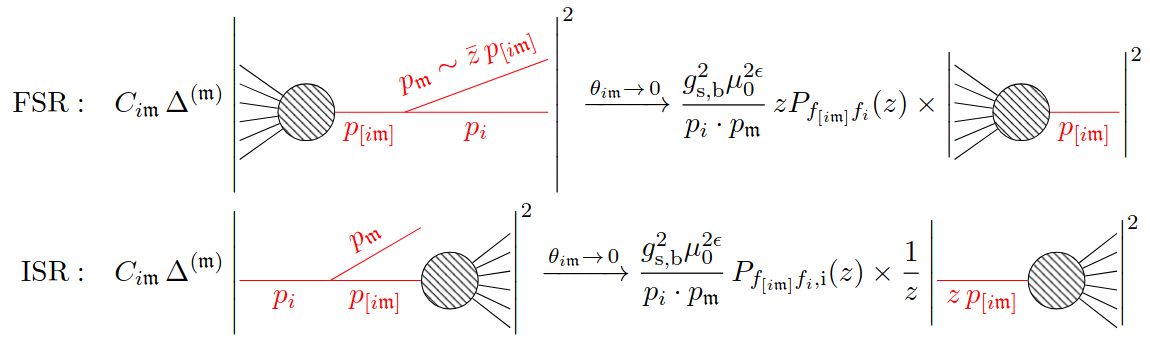
\includegraphics[width=1.0\textwidth]{imgs/splitting.png}
	\caption{Graphical representation of the convention used for collinear factorization. The upper diagram illustrates the final-state splitting process, whereas the lower diagram represents the initial-state splitting process. We observe that for Final-State Radiation (FSR), the action of the operator $C_{i\um}$ on $\Delta^{(\um)}$ introduces an additional factor of $z$, a feature that is absent in Initial-State Radiation (ISR). Figure from \cite{Devoto:2025kin}.}
	\label{hadron-collision-pict}
\end{figure}


\subsection{Initial state}
\label{initial-state-section}
We consider the situation where a gluon $\um$ in the final state becomes collinear to a quark $a$ in the initial state. This could happen, for instance, in the case of process $\mathcal{P}_1^{\mathrm{NLO}}$. The squared matrix element, which is used to define the function $F_{\mathrm{LM}}$, has a dependence on the energy fraction variable $z=1-E_\um/E_a$. As a direct consequence of this dependence, the integral over the collinear gluon's energy cannot be performed. Nevertheless, we can still carry out the angular integration over the relative angle between the emitted gluon $\um$ and the incoming parton $a$. \\
We begin by examining how the cross section factorizes upon the application of the collinear operator
\begin{equation}
  C_{a\um} \Delta^{(\um)} F_{\mathrm{LM}} = \frac{g^2_{s,b}}{p_a \cdot p_\um} \frac{P_{qq}(z)}{z} F_{\mathrm{LM}}(z\cdot a_q) \, ,
\end{equation}
where $z \cdot a_q$ denotes a quark whose momentum is the product of $z$ and the momentum of the incoming quark $a$. We emphasize that this relationship is the fundamental reason we cannot integrate over $E_\um$. The corresponding splitting function for this limit is
\begin{equation}
  P_{qq}(z) = C_F \left[\frac{1+z^2}{1-z}-\epsilon(1-z)\right]\, .
\end{equation}
If, instead, both the soft and collinear operators are applied, one obtains
\begin{equation}
  C_{a\um} S_{\um} F_{\mathrm{LM}} (a_q, \um) = \lim_{z \to 1}  C_{a\um} F_{\mathrm{LM}} (a_q, \um)= \frac{g^2_{s,b}}{p_a \cdot p_\um} \frac{2 C_F}{1-z} F_{\mathrm{LM}}( a_q) \, .
\end{equation}
Also in this case, it is convenient to perform the integration in hyperspherical coordinates. Furthermore, it is useful to implement a change of variables by parametrizing the gluon energy as $E_\um = (1-z)E_a$, which implies that the measure transforms as $\mathrm{d}E_\um=-E_a \mathrm{d}z$. Therefore, Eq. \ref{measure-ps} becomes
\begin{equation}
  [\mathrm{d}p_\um] = \frac{E_a^{d-2}\, (1-z)^{d-3} \, \mathrm{d}z \, \mathrm{d}\Omega ^{d-1}}{2 \, (2\pi)^{d-1}} \theta(z-z_{\mathrm{min}}) \, ,
\end{equation}
where $z_{\mathrm{min}} = 1 - E_{\mathrm{max}}/E_a$, and $d=4-2\epsilon$. We also note that $p_a \cdot p_\um = E_a E_\um \rho_{a\um}=(1-z)E_a^2\rho_{a \um}$. We can therefore proceed with the integration. For the moment, we will only explicitly perform the phase space integration for parton $\um$
\begin{equation}
  \begin{split}
  & \int [\mathrm{d}p_\um] \, C_{a\um} \bar{S}_\um F_{\mathrm{LM}} (a_q, \um) = \\
  & = g^2_{s,b}  \int \frac{\mathrm{d}\Omega ^{d-1}}{2 (2\pi)^{d-1}} \, E_a^{-2\epsilon} \int_{z_{\mathrm{min}}}^{1} \mathrm{d}z (1-z)^{-2\epsilon} \frac{1}{ \rho_{a \um}} \left[\frac{P_{qq}(z)}{z} F_{\mathrm{LM}}(z \cdot a_q) - \frac{2 C_F}{1-z}F_{\mathrm{LM}} (a_q) \right] \, .
  \label{coll-pass}
  \end{split}
\end{equation}
Now we solve the angular integral using the following equation, Eq. G.5 in \cite{Asteriadis:1910}
\begin{equation}
  \int \frac{\mathrm{d}\Omega ^{d-1}}{2 (2\pi)^{d-1}} \frac{1}{\rho_{a \um}}= -\frac{2^{-2\epsilon}}{\epsilon} \left[ \frac{(4\pi)^{\epsilon}}{8\pi^2 \, \Gamma(1-\epsilon)}\right] \left[\frac{\Gamma^2(1-\epsilon)}{\Gamma(1-2\epsilon)} \right] \, .
  \label{angular-integral}
\end{equation}
Moreover, we use the shorthand notation $[\alpha_s]$ in Eq. \ref{coupling}. Thus, Eq. \ref{coll-pass} becomes
\begin{equation}
  \begin{split}
  & \int [\mathrm{d}p_\um] \, C_{a\um} \bar{S}_\um \Delta^{(\um)} F_{\mathrm{LM}} (a_q, \um) = \\
  & = [\alpha_s] \left(-\frac{1}{\epsilon}\right) \left(\frac{4E_a^2}{\mu^2}\right)^{-\epsilon} \frac{\Gamma^2(1-\epsilon)}{\Gamma(1-2\epsilon)} \int_{z_{\mathrm{min}}}^{1} \mathrm{d}z (1-z)^{-2\epsilon} \left[ \frac{P_{qq}(z)}{z} F_{\mathrm{LM}}(z \cdot a_q) - \frac{2 C_F}{1-z}F_{\mathrm{LM}} (a_q) \right] \,.
  \label{coll-pass-1}
  \end{split}
\end{equation}
According to the momentum conservation constraint in Eq. \ref{leading-order}, $E_{\max}$ must be greater than or equal to the maximum energy that a final-state parton can carry. Consequently, $E_{\max} \geq E_a$ and thus $z_{\mathrm{min}} \leq 0$. This implies that $F_{\mathrm{LM}}(z \cdot a_q) = 0$ for $z \in \big[z_{\mathrm{min}}, 0 \big)$,  while the lower limit of integration on the second-term of Eq. \ref{coll-pass-1} remains $z_{\mathrm{min}}$. Furthermore, in $P_{qq}$, we isolate the term that is singular in the $z \to 1$ limit in the following way
\begin{equation}
  P_{qq}(z) = \frac{2 C_F}{1-z} + P_{qq,\mathrm{reg}} (z), \qquad P_{qq,\mathrm{reg}} (z) = - C_F [(1+z)+\epsilon(1-z)] \, ,
\end{equation}
and write
\begin{equation}
  \begin{split}
  & \int [\mathrm{d}p_\um] \, C_{a\um} \bar{S}_\um \Delta^{(\um)} F_{\mathrm{LM}} (a_q, \um) = \\
  & = -\frac{[\alpha_s]}{\epsilon}  \left(\frac{2E_a}{\mu}\right)^{-2\epsilon} \frac{\Gamma^2(1-\epsilon)}{\Gamma(1-2\epsilon)} \Biggl\{ \int_{0}^{1} \mathrm{d}z \Biggl[  \left( \frac{2C_F}{(1-z)^{1+2\epsilon}} + \frac{P_{qq, \mathrm{reg}}(z)}{(1-z)^{2\epsilon}} \right) \times \\
  & \times \frac{F_{\mathrm{LM}}(z\cdot a_q)}{z} - \frac{2 C_F}{(1-z)^{1+2\epsilon}} F_{\mathrm{LM}}(a_q) \Biggr] + C_F \frac{(E_{\mathrm{max}}/E_a)^{-2\epsilon}-1}{\epsilon} F_{\mathrm{LM}}(a_q)  \Biggr\} \,.
  \label{coll-pass-1}
  \end{split}
\end{equation}
Now we identify $G(z)=F_{\mathrm{LM}}(z \cdot a_q)/z$, and use the definition of the plus distribution
\begin{equation}
  \frac{1}{(1-z)^{1+2\epsilon}} = \sum_{n=0}^{\infty} \frac{(-2\epsilon)^n}{n!} \frac{\log^n{(1-z)}}{1-z} \,,
\end{equation}
and the following equation
\begin{equation}
  \int_0^1 \mathrm{d}z \, \mathcal{D}_n(z) G(z) = \int_0^1 \mathrm{d}z \frac{\log^n{(1-z)}}{1-z} \, \left(G(z)-G(1)\right) \, ,
\end{equation}
and we obtain 
\begin{equation}
  \begin{split}
  & \int [\mathrm{d}p_\um]\, C_{a\um} \bar{S}_\um \Delta^{(\um)} F_{\mathrm{LM}} (a_q, \um) = \\
  & = -\frac{[\alpha_s]}{\epsilon}  \left(\frac{2E_a}{\mu}\right)^{-2\epsilon} \frac{\Gamma^2(1-\epsilon)}{\Gamma(1-2\epsilon)} \Biggl\{ \int_0^1 \frac{\mathrm{d}z}{(1-z)^{2\epsilon}} P_{qq,\mathrm{reg}(z)} \frac{F_{\mathrm{LM}}(z\cdot a_q)}{z} + \\
  & + 2C_F \sum_{n=0}^{\infty} \frac{(-2\epsilon)^n}{n!} \int_0^1 \mathrm{d}z \, \mathcal{D}_n(z) \, \frac{F_{\mathrm{LM}}(z\cdot a_q)}{z} + \int_0^1 C_F \frac{(E_{\mathrm{max}}/E_a)^{-2\epsilon}-1}{\epsilon} F_{\mathrm{LM}}(a_q) \Biggr\} \, .  
  \label{coll-pass-2}
  \end{split}
\end{equation}
Moreover, we introduce the following definition
\begin{equation}
  \hat{P}_{qq}^{(0)}(z) = C_F \left[ 2 \mathcal{D}_0 (z)-(1+z)+\frac{3}{2} \delta(1-z) \right],
  \label{kernel-pqq}
\end{equation}
that is the leading-order Altarelli-Parisi splitting kernel (see Eq. \ref{altarelli-parisi}), and
\begin{equation}
  \mathcal{P}_{qq}^{\mathrm{fin}}= - \frac{C_F}{\epsilon} \left[2 \sum_{n=1}^{\infty} \frac{(-2\epsilon)^n}{n!} \, \mathcal{D}_n(z)+(1-z)^{-2\epsilon} \, P_{qq, \mathrm{reg}}(z)+(1-z) \right] \, .
  \label{P-qq-finite}
\end{equation}
These quantities appear in the definition of the \emph{generalized splitting function}, which allows us to express the result in a more compact form
\begin{equation}
  \mathcal{P}_{qq}^{\mathrm{gen}} = \left(\frac{2E_a}{\mu}\right)^{-2\epsilon} \frac{\Gamma^2(1-\epsilon)}{\Gamma(1-2\epsilon)} \left[-P^{(0)}_{qq}+\epsilon \mathcal{P}_{qq}^{\mathrm{fin}}\right] \, .
  \label{gen-splitt-funct}
\end{equation}
It is also useful to introduce the \emph{generalized initial-state anomalous dimension}, which reads
\begin{equation}
  \Gamma_{a,q} = \left(\frac{2E_a}{\mu}\right)^{-2\epsilon} \frac{\Gamma^2(1-\epsilon)}{\Gamma(1-2\epsilon)} \left(\gamma_q + \vec{T}_q^2 \,\frac{1-e^{-2\epsilon L_a}}{\epsilon}\right) \, ,
  \label{generalized-anom-dim}
\end{equation}
where $\gamma_q$ is the anomalous dimension of the initial-state parton $a=q$, which can be found in Appendix \ref{anomalous-dimension}, and $L_a =\log{(E_{\mathrm{max}}/E_a)}$. Therefore, the integrated hard-collinear counterterm for a gluon $\um$ going collinear to a quark $a$ in the initial state reads
\begin{equation}
  \left< C_{a\um} \bar{S}_\um \Delta^{(\um)} F_{\mathrm{LM}} (\um) \right> = [\alpha_s] \left< \frac{\Gamma_{a,q}}{\epsilon} F_{\mathrm{LM}} \right> + \frac{[\alpha_s]}{\epsilon}\left< \mathcal{P}_{qq}^{\mathrm{gen}} \otimes F_{\mathrm{LM}} \right> \, ,
  \label{initial-state-collinear}
\end{equation}
where we also used the shorthand notation
\begin{equation}
  \mathcal{P}_{qq}^{\mathrm{gen}} \otimes F_{\mathrm{LM}} = \int_0^1 \, \mathrm{d}z \, \mathcal{P}_{qq}^{\mathrm{gen}}(z) \, \frac{F_{\mathrm{LM}}(z \cdot a_q)}{z} \, .
  \label{convolution}
\end{equation}
\\
Let us now consider the situation where a final-state gluon $\um$ becomes collinear with an initial-state gluon $a$. The calculation remains analogous to the previous case, but the form of some functions changes. Specifically, the splitting function is now $P_{gg}$, whose expression is given in Eq. \ref{splitting-functions} and illustrated in Fig.\ref{hadron-collision-pict}. Furthermore, the leading-order Altarelli-Parisi splitting kernel is now $\hat{P}_{gg}^{(0)}(z)$, reported in \ref{altarelli-parisi}. The integrated hard-collinear counterterm in this case has the same form as in Eq. \ref{initial-state-collinear}, but uses the generalized anomalous dimension for a gluon $\Gamma_{a,g}$ (defined as in \ref{generalized-anom-dim}, with $g$ in place of $q$), and the term from Eq. \ref{convolution} now involves the generalized splitting function $\mathcal{P}_{gg}^{\mathrm{gen}}$. This function has the form \ref{gen-splitt-funct}, adapted for the case of a gluon collinear to another gluon. \\

Finally, we consider the case where a final-state quark $\um$ becomes collinear with another initial-state parton $a$, which can be either a quark or a gluon. As stated previously, quarks do not give rise to soft singularities. Therefore, in this scenario, the term involving the anomalous dimension in Eq. \ref{initial-state-collinear} is absent. Only the generalized splitting function remains, which can be obtained from Eq. \ref{kernel-pqq} by replacing $qq$ with $qg$ in the case of a quark becoming colliner to a initial state gluon, and $qq$ with $gq$ in the case of a quark becoming collinear to an initial state quark (see Fig. \ref{hadron-collision-pict})". \\

We can summarize these results with a general expression for the soft-regulated initial state collinear terms
\begin{equation}
  \left< C_{a\um} \bar{S}_\um \Delta^{(\um)} F_{\mathrm{LM}} (\um) \right> = [\alpha_s] \left< \frac{\Gamma_{1,a}}{\epsilon} F_{\mathrm{LM}} \right> + \frac{[\alpha_s]}{\epsilon}\left< \mathcal{P}_{aa}^{\mathrm{gen}} \otimes F_{\mathrm{LM}} \right> \, ,
  \label{initial-state-collinear}
\end{equation}
where $\Gamma_{1,a}$ is defined as in Eq. \ref{generalized-anom-dim}, replacing $q$ with the specific parton considered.

\subsection{Final state}
\label{final-state-section}
Let us now consider a situation where a final-state gluon $\um$ becomes collinear with another final-state gluon $i$. This can occur, for example, in the case of the $\mathcal{P}_2^{\mathrm{NLO}}$ process. In this case, the function $F_{\mathrm{LM}}$ depends on the energy fraction $z=1-E_\um/E_{i\um}=E_i/E_{i\um}$, and, under the action of the collinear operator, it factorizes in the following way
\begin{equation}
  C_{i \um} \Delta^{(\um)} F_{\mathrm{LM}} (\um) = \frac{g^2_{s,b}}{p_i \cdot p_\um} z P_{gg}(z) F_{\mathmakebox{LM}}(i\um)\, ,
  \label{collinear-factorization}
\end{equation}
where the argument of the function $F_{LM}$ on the right-hand side shows the dependence on the momentum of the single final-state gluon $[i\um]$ resulting from the merging of the two collinear gluons, and
\begin{equation}
  P_{gg}(z)= 2C_A \left[ \frac{z}{1-z}+\frac{1-z}{z}+z(1-z)\right] \, .
\end{equation}
We perform the integration in hyperspherical coordinates over the phase space of the gluons involved in the collinear limit, namely $i$ and $\um$. To facilitate the subsequent change of variables, we isolate, from the angular integral, the integration over the relative angle between partons $i$ and $\um$, i.e., $\theta_{[i\um]}$, and in particular we highlight the variable $\eta_{i\um}=\rho_{i\um}/2$
\begin{align}
  \int [\mathrm{d}p_i] \int [\mathrm{d}p_\um] \, C_{i\um} \Delta^{(\um)} F_{\mathrm{LM}} 
  &= \int \frac{\mathrm{d}\Omega^{d-2}}{2(2\pi)^{d-1}} 2^{-2\epsilon} \int_0^1 \frac{\mathrm{d}\eta_{i\um}}{(\eta_{i\um}(1-\eta_{i\um}))^{\epsilon}} \nonumber \\
  &\quad \times \int [\mathrm{d}\Omega_i] \int \mathrm{d}E_\um E_\um^{1-2\epsilon} \int \mathrm{d}E_i E_i^{1-2\epsilon} 
  \frac{g_{s,b}^2 P_{gg} F_{\mathrm{LM}} (i\um) }{(1-z) E_{i\um}^{2}\eta_{i\um}} .
\end{align}
We now employ the following integrals
\begin{equation}
  \int \frac{\mathrm{d}\Omega^{d-2}}{2(2\pi)^{d-1}} = \frac{1}{8\pi^2} \frac{(4\pi)^{\epsilon}}{\Gamma(1-\epsilon)} \, , \qquad \int_0^1 \frac{\mathrm{d}\eta_{i\um}}{(\eta_{i\um}(1-\eta_{i\um}))^{\epsilon}} \frac{1}{\eta_{i\um}} = - \frac{1}{\epsilon} \frac{\Gamma^2(1-\epsilon)}{\Gamma(1-2\epsilon)} \, , 
\end{equation}
and the abbreviated notation $[\alpha_s]$. Furthermore, as anticipated, we perform a change of variables: from integration in $\mathrm{d}E_i$ and $\mathrm{d}E_\um$, which had the integration range $[0,E_{\mathrm{max}}]\times [0,E_{\mathrm{max}}]$, we move to the variables $z$ and $E_{i\um}$, in the range $[1,z_{\mathrm{min}}]\times [0,E_{\mathrm{max}}]$, with $z_{\mathrm{min}}=1-E_{\mathrm{max}}/E_{i\um}$. We thus obtain
\begin{align}
  \int [\mathrm{d}p_i] \int [\mathrm{d}p_\um] \, C_{i\um} \Delta^{(\um)} F_{\mathrm{LM}} 
  &= [\alpha_s] \mu^{2\epsilon}2^{-2\epsilon}\left[- \frac{1}{\epsilon} \frac{\Gamma^2(1-\epsilon)}{\Gamma(1-2\epsilon)} \right] \int [\mathrm{d}\Omega_i]\int_0^{E_{\mathrm{max}}} \mathrm{d}E_{i\um} \nonumber \\
  &\quad \times \int_{z_{\mathrm{min}}}^{1} \mathrm{d}z \, z^{1-2\epsilon} \, E_{i\um}^{1-4\epsilon} \,(1-z)^{-2\epsilon}P_{gg}(z)F_{\mathrm{LM}}(i\um) .
\end{align}
Now, we rename the variable $[i\um]$ as $i$. Furthermore, we observe that the function $F_{\mathrm{LM}}(i\um)=F_{\mathrm{LM}}(z^{-1}\cdot i)$ depends on $z$ and that $z_{\mathrm{min}}\leq0$, due to the same arguments we made earlier. Therefore, we can state that $F_{\mathrm{LM}}(z \cdot a_q) = 0$ for $z \in [z_{\mathrm{min}}, 0)$. We thus obtain
\begin{equation}
  \begin{split}
  & \int [\mathrm{d}p_i] \int [\mathrm{d}p_\um] \, C_{i\um} \Delta^{(\um)} F_{\mathrm{LM}} = \\
  & = [\alpha_s] \, \frac{1}{\epsilon} \int[\mathrm{d}p_i] \left(\frac{2E_i}{\mu} \right)^{-2\epsilon} \frac{\Gamma^2(1-\epsilon)}{\Gamma(1-2\epsilon)} \cdot \left( - \int_0^1 \mathrm{d}z \, z^{1-2\epsilon} \, (1-z)^{-2\epsilon} \, P_{gg}(z)\right) \, F_{\mathrm{LM}} .
  \end{split}
\end{equation}
In constrast to the initial state case, the function $F_{\mathrm{LM}}$ does not depend on $z$, and hence the integral over this variable can be performed. We now add the soft-collinear term. Since the limit $E_{\um} \to 0$ is equivalent to $z \to 1$, we express the soft operator as $S_z$. We observe that, after applying the soft limit, the function $F_{\mathrm{LM}}$ does not depend on $z$, and therefore we cannot use the same argument as before to restrict the integration range. However, we can rewrite the integral over the interval $[z_{\mathrm{min}},1]$ as an integral over $(0,1]$ minus the integral over $(0,z_{\mathrm{min}}]$. By doing so, we obtain
\begin{align}
  \int [\mathrm{d}p_i] \int [\mathrm{d}p_\um] \, C_{i\um} S_{\um} \Delta^{(\um)} F_{\mathrm{LM}} 
  &= [\alpha_s] \, \frac{1}{\epsilon} \int[\mathrm{d}p_i] \left(\frac{2E_i}{\mu} \right)^{-2\epsilon} \frac{\Gamma^2(1-\epsilon)}{\Gamma(1-2\epsilon)} \nonumber \\
  & \times \left[ - \int_0^1 \mathrm{d}z \, S_z \, z^{1-2\epsilon} (1-z)^{-2\epsilon} P_{gg}(z) - \frac{C_A}{\epsilon} \left(1-\frac{E_{\text{max}}}{E_i}\right) \right] F_{\mathrm{LM}} .
\end{align}
Putting together the obtained results, the integrated hard-collinear counterterm for a gluon $\um$ going collinear to a quark $i$ in the final state reads
\begin{equation}
  \left<  C_{i\um} \bar{S}_{\um} \Delta^{(\um)} F_{\mathrm{LM}}\right> = \frac{[\alpha_s]}{\epsilon} \left< \Gamma_{i,g \to gg} \, F_{\mathrm{LM}}\right> \, ,
\end{equation}
where $\Gamma_{g,g \to gg}$ is the \emph{weighted final-state anomalous dimension}, which, in the general case, has the form
\begin{equation}
  \Gamma_{i,f_{[i\um]}\to f_i f_\um} = \left[\left(\frac{2E_i}{\mu}\right)^{-2\epsilon} \frac{\Gamma^2(1-\epsilon)}{\Gamma(1-2\epsilon)}\right] \, \gamma^{22}_{z,f_{[i\um]} \to f_i f_\um} (L_i) \, ,
  \label{gen-final-anom-dim}
\end{equation}
where 
\begin{align}
  \gamma^{nk}_{g(z),f_{[i\um]}} (L_i) 
  &= - \int_0^1 \mathrm{d}z \, \bar{S}_z \left[z^{-n\epsilon}(1-z)^{-k\epsilon}g(z)P_{f_{[i\um]}f_i}(z)\right] \nonumber \\
  &\quad + 2 \delta_{f_{[i\um]}f_i} \vec{T}^2_{f_{[i\um]}} \frac{1-e^{-k \epsilon L_i}}{k\epsilon} g(1) ,
  \label{gen-an-dim}
\end{align}
and $L_i=\log{\left(E_{\mathrm{max}}/E_i\right)}$. We observe that the quantity in Eq. \ref{gen-final-anom-dim} differs from the conventional collinear anomalous dimension that arises from integrals of the collinear splitting functions without additional factors of $z=z_{i,\um}$. Furthermore, the expansion in $\epsilon$ of $\Gamma_{g,g \to gg}$ is $\Gamma_{g,g \to gg}=\frac{11}{6}C_A+2C_AL_i+\mathcal{O}(\epsilon)$, which yields exactly the term proportional to $C_A$ in the gluon anomalous dimension but lacks the term proportional to $n_f$, i.e., the number of quark flavours. To see how the conventional collinear anomalous dimension emerges, we need to consider the contribution from other two partons becoming collinear: when an unresolved (anti)quark $\um$ goes collinear to another (anti)quark $i$ in the final state. The calculation in this case is identical to the previous one, with the difference that $S_q = 0$, and with the splitting function $P_{gq}(z)$ (see \ref{splitting-functions} and Fig. \ref{hadron-collision-pict}). Therefore, the second term on the right-hand side of Eq. \ref{gen-an-dim} vanishes: indeed, $f_{[i\um]}=g$ and $f_i=q$, hence $\delta_{f_{[i\um]}f_i}=0$. Due to the symmetries of the splitting and the fact that it does not depend on the quark flavour\footnote{For details, see Section 3 of \cite{Devoto:2025kin}.}, this contribution is given by the corresponding result multiplied by a factor of $2n_f$.
\begin{equation}
  \left<  C_{i\um} \bar{S}_{\um} \Delta^{(\um)} F_{\mathrm{LM}}\right> = \frac{[\alpha_s]}{\epsilon} \left< 2n_f \, \Gamma_{i,g \to q \bar{q}} \, F_{\mathrm{LM}}\right> \, .
\end{equation}
The sum of the two contributions allows us to recover the generalized collinear anomalous dimension, which we define as
\begin{equation}
  \Gamma_{i,g} = \Gamma_{i,g \to gg} + 2n_f \Gamma_{i,g \to q \bar{q}} \, ,
  \label{an-dim-gluon}
\end{equation}
which, when expanded in $\epsilon$, takes the form 
\begin{equation}
  \Gamma_{i,g}=\gamma_g + 2 \vec{T}_g^2 L_i + \mathcal{O}(\epsilon) \, ,
  \label{expansion-an-dim-gluon}
\end{equation}
and contains precisely the conventional gluon anomalous dimension $\gamma_g$. \\

We are left to analyze the cases in which a gluon $\um$ becomes collinear to a quark $i$ in the final state, and the opposite case, i.e., in which a quark $\um$ becomes collinear to a quark $i$ in the final state. Again, the calculations are analogous to to those presented above, but the splitting functions differ: when a gluon $\um$ is collinear to a quark $i$, one uses $P_{qq}(z)$, while in the opposite case one uses $P_{qg}(z)$, both of which can be found in Eq. \ref{splitting-functions} and Fig. \ref{hadron-collision-pict}. Also in this latter case, the soft limit is absent, and the delta function in \ref{gen-an-dim} vanishes. To obtain the conventional collinear anomalous dimension, it is again necessary to sum the two contributions, yielding
\begin{equation}
  \Gamma_{i,q} = \Gamma_{i,q \to qg} + \Gamma_{i,q \to gq} \,.
  \label{an-dim-quark}
\end{equation}
This quantity can be expanded  in $\epsilon$ as 
\begin{equation}
  \Gamma_{i,q} = \gamma_q+ 2 C_F L_i + \mathcal{O}(\epsilon) \,. 
  \label{expansion-an-dim-quark}
\end{equation}
What allows us to recover the conventional quark anomalous dimension is the fact that the weight factors $z_{i\um}$ cancel out when combining the two splittings \cite{Devoto:2025kin}. 


\subsection{Hard-collinear operator}
The study of all possible combinations of partons that can become collinear allows us to express the integrated soft-collinear counterterm in a general form, which reads
\begin{equation}
  \left< \bar{S}_{i\um} C_{i\um} \Delta^{(\um)} F_{\mathrm{LM}}(\um)\right> = [\alpha_s] \left< I_{\mathrm{C}}(\epsilon) \cdot F_{\mathrm{LM}} \right> + \frac{[\alpha_s]}{\epsilon} \left[\left< P_{aa}^{\mathrm{gen}} \otimes F_{\mathrm{LM}} \right> + \left< F_{\mathrm{LM}} \otimes P_{bb}^{\mathrm{gen}}  \right>\right] \, , 
  \label{soft-collinear-integrated}
\end{equation}
where $a$ and $b$  indicate the initial-state partons, and where we have introduced the hard collinear operator
\begin{equation}
  I_{\mathrm{C}}(\epsilon) = \sum_{i=1}^{N_p} \frac{\Gamma_{i,f_i}}{\epsilon}  \, ,
  \label{IC-def}
\end{equation}
with $N_p$  being the total number of partons involved.

\section{Cancellation of poles}
\label{pole-cancellation-section}
Having determined the general form of the operators $I_{\mathrm{S}}(\epsilon)$ and $I_{\mathrm{C}}(\epsilon)$, we can now show that the total operator $I_{\mathrm{T}} (\epsilon)=I_{\mathrm{S}}(\epsilon)+I_{\mathrm{C}}(\epsilon)+I_{\mathrm{V}}(\epsilon)$ is finite as $\epsilon \to 0$, meaning that all the poles in $\epsilon$ cancel\footnote{Details can be found in Appendix C of \cite{Devoto:2025kin}.}. To do this, we expand the various operators in powers of $\epsilon$ and then perform the sum. \\

We start with the soft operator $I_{\mathrm{S}}(\epsilon)$ defined in Eq.~\ref{I-s-operator}. For the purpose of its expansion, we define the following function
\begin{equation}
  f_k(x) = \frac{x^{-k\epsilon}-1}{\epsilon} \, ,
\end{equation}
which satisfies $f_k(x) \sim \mathcal{O}(\epsilon^0) $. This definition is particularly useful because it makes explicit that the $\epsilon$-expansion of factors like $(2E_{\mathrm{max}}/\mu)^{-\epsilon}$ and $\eta_{ij}^{-\epsilon}$ begins at $1$. Furthermore, we employ the following expansion for the function $K_{ij}$ defined in Eq. \ref{k-function}
\begin{equation}
  K_{ij} = 1+ K_{ij}^{(2)} \epsilon^2 + \mathcal{O}(\epsilon^3) \, , \qquad  K_{ij}^{(2)} = \mathrm{Li}_2(1-\eta_{ij}) - \frac{\pi^2}{6} \, , 
\end{equation}
and we obtain 
\begin{equation}
  I_{\mathrm{S}}(\epsilon) = - \frac{1}{\epsilon^2} \left[1+\epsilon f_2 \left(\frac{2 E_{\mathrm{max}}}{\mu}\right)\right] \sum_{i \neq j}^{N_p} (1+\epsilon f_1(\eta_{ij}))(1+ \epsilon^2 K_{ij}^{(2)} + \mathcal{O}(\epsilon^3)) \left( \vec{T}_i \cdot \vec{T}_j\right) \,.
\end{equation}
At this stage, we have neglected terms of $\mathcal{O}(\epsilon)$ in the overall prefactor. Since we are ultimately interested in terms up to $\mathcal{O}(\epsilon^0)$, this expression can be simplified further
\begin{equation}
  \begin{aligned}
   I_{\mathrm{S}}(\epsilon) & = - \frac{1}{\epsilon^2} \left[1+\epsilon f_2 \left(\frac{2 E_{\mathrm{max}} }{\mu}\right)\right] \sum_{i \neq j}^{N_p}\left( \vec{T}_i \cdot \vec{T}_j\right) - \frac{1}{\epsilon} \sum_{i \neq j}^{N_p} f_1(\eta_{ij}) \left( \vec{T}_i \cdot \vec{T}_j\right)  \\
  & - \sum_{i \neq j}^{N_p} \left[f_2 \left(\frac{2 E_{\mathrm{max}} }{\mu}\right) f_1(\eta_{ij}) + K_{ij}^{(2)} \right] \left( \vec{T}_i \cdot \vec{T}_j\right) + \mathcal{O}(\epsilon) \, . 
  \end{aligned}
\end{equation}
We can further simplify terms where only the color charge operators depend on the summation indices $i$ and $j$. In such cases, the summation over one of the indices can be performed by exploiting color conservation. This fundamental property, which holds for the color-space vector $\ket{\mathcal{M}}_c$ of any QCD amplitude, is expressed as
\begin{equation}
  \sum_{k=1}^{N_p} \vec{T}_k  \ket{\mathcal{M}}_c = 0 \, .
\end{equation}
A detailed treatment of this formalism can be found in Ref. \cite{Catani:1996vz}. It follows that 
\begin{equation}
  \sum_{k=1}^{N_p} \, {}_c \bra{\mathcal{M}} \left( \vec{T}_i \cdot \vec{T}_j\right) \ket{\mathcal{M}} {}_c= - \vec{T}^2_i |\mathcal{M}|^2 \, ,
  \label{color-conservation}
\end{equation}
and we obtain
\begin{equation}
  \begin{aligned}
  I_{\mathrm{S}}(\epsilon)  &= \sum_{i=1}^{N_p}  \left[1+\epsilon f_2(2E_{\mathrm{max}}/\mu)\right] \frac{\vec{T}_i^2}{\epsilon^2}- \sum_{i\neq j}^{N_p} \frac{f_1(\eta_{ij})}{\epsilon} \left( \vec{T}_i \cdot \vec{T}_j\right) \\
 & - \sum_{i\neq j}^{N_p} \left[ f_2 \left(2 E_{\mathrm{max}}\right) f_1(\eta_{ij}) + K_{ij}^{(2)}\right] (\vec{T}_i \cdot \vec{T}_j) + \mathcal{O}(\epsilon) \,.
  \end{aligned}
\end{equation}
The terms in the last line are finite as $\epsilon \to 0$. To cancel the divergent terms, however, we must sum the contributions from the other operators. Regarding the virtual corrections, it is useful to introduce an operator $I_{\mathrm{V}}(\epsilon)$, based on Catani's formula for the infrared poles of one-loop amplitudes \cite{Catani:1998bh} and following the procedure outlined in \cite{Devoto:2023rpv}
\begin{equation}
  I_{\mathrm{V}}(\epsilon) = \bar{I}_1 (\epsilon) + \bar{I}_1\textsuperscript{\textdagger} (\epsilon) \,, \qquad \bar{I}_1 (\epsilon)= \frac{1}{2} \sum_{(ij)}^{N_p} \frac{\mathcal{V}_i^{\mathrm{sing}}(\epsilon)}{\vec{T}_i^2} \left( \vec{T}_i \cdot \vec{T}_j\right) \left(\frac{\mu^2}{2p_i \cdot p_j}\right)^{\epsilon} e^{i \pi \lambda_{ij} \epsilon} \, ,
\end{equation}
where the parameters $\lambda_{ij}$ are $1$ if $i$ and $j$ are both incoming or outgoing partons, and zero otherwise, and 
\begin{equation}
  \mathcal{V}_i^{\mathrm{sing}}= \frac{\vec{T}_i^2}{\epsilon^2} + \frac{\gamma_i}{\epsilon} \,. 
\end{equation}
Using the same property as in Eq.~\ref{color-conservation}, it is also possible to expand the operator $I_{\mathrm{V}}(\epsilon)$ in powers of $\epsilon$. By summing the soft and virtual operators, we obtain
\begin{equation}
  I_{\mathrm{S}}(\epsilon)+I_{\mathrm{V}}(\epsilon)= - \frac{1}{\epsilon} \sum_{i=1}^{N_p} \left[2 L_i \vec{T}_i^2 + \gamma _i\right] + \mathcal{O}(\epsilon^0)\, .
  \label{IsIv-sum}
\end{equation}
Thus, we observe that the summation of the soft and virtual operators results in the cancellation of the $1/\epsilon^2$ poles, while single poles in $1/\epsilon$ persist. These remaining divergences are expected to cancel against contributions from the $I_{\mathrm{C}}(\epsilon)$ operator. This expectation is indeed confirmed by explicit calculation. Specifically, considering the definition of the operator in Eq.~\ref{IC-def} and employing the expansions of the generalized collinear anomalous dimensions given in Eqs.~\ref{expansion-an-dim-gluon} and \ref{expansion-an-dim-quark}, the operator $I_{\mathrm{C}}(\epsilon)$ can be expanded in powers of $\epsilon$ as follows
\begin{equation}
  I_{\mathrm{C}}(\epsilon)= \frac{1}{\epsilon}\sum_{i=1}^{N_p} \left( 2 L_i \vec{T}_i^2 + \gamma _i \right) + \mathcal{O}(\epsilon^0)\, .
  \label{Ic-expanded}
\end{equation}
From the comparison of Eqs.~\ref{IsIv-sum} and \ref{Ic-expanded}, it is clear that the operator $I_{\mathrm{T}}(\epsilon)$ is finite. Furthermore, as demonstrated in \cite{Devoto:2025kin}, the initial-state singularities present in Eq.~\ref{initial-state-collinear} also cancel, due to the singular terms in the PDFs renormalization and exploiting the relation $\mathcal{P}_{ab}^{\mathrm{gen}}+\hat{P}_{ab}(0) \sim \mathcal{O}(\epsilon)$, where $\hat{P}_{ab}(0)$ are the Altarelli-Parisi splitting functions.

\clearpage

\chapter{NLO QCD corrections with $\theta$-parameters in the NSC Subtraction Scheme}
\label{NSC-SS-parameters}
Among the criteria used to evaluate the quality of a subtraction scheme are computational efficiency and numerical stability in the evaluation of the physical results (such as cross sections and differential distributions) that are produced. This is critically important because the complex processes that take place at the LHC, involving high-multiplicity final states, require sophisticated numerical integration over particularly large and complex phase spaces. To have greater control over this integration, ensure that we are sampling the smallest and most physically relevant phase space possible, and minimize the computational cost, it is convenient to introduce a set of tunable parameters into the NSC Subtraction Scheme. These parameters allow us to modulate the boundaries of the soft and collinear regions, effectively controlling the integration limits we use.

\section{Processes}
Before delving into the technical details of the parameter implementation, we first describe the class of processes for which we will derive and show the explicit form of the subtraction terms. Following the scheme of the papers \cite{Devoto:2023rpv,Devoto:2025kin}, we will now consider processes that are more general than the illustrative examples introduced in Section \ref{modularity-scheme}. In particular, as in \cite{Devoto:2023rpv}, we will begin by considering the production of an arbitrary number of gluons and a colorless final state $X$ in $q \bar{q}$ annihilation, thus restricting ourselves to the case where all resolved and unresolved final-state partons are gluons. At leading-order, we write this process as

\begin{equation}
  \mathcal{A}^{\mathrm{LO}}: \quad a_q + b_{\bar{q}} \to X + N \, g \, ,
\end{equation}
where $N$ is the number of produced jets. The NLO cross section for this process receives a real-emission contribution from the process
\begin{equation}
  \mathcal{A}^{\mathrm{NLO}}: \quad a_q + b_{\bar{q}} \to X + (N+1) \, g \, .
\end{equation}
Then, to proceed with the generalization of the scheme, we will analyze, as in \cite{Devoto:2025kin}, the partonic channel whose leading-order process has the form \cite{Devoto:2025kin}
\begin{equation}
  \mathcal{B}^{\mathrm{LO}}: \quad a_g + b_q \to X + N_g \, g + q \, ,
\end{equation}
where $N_g=N-1$. This configuration receives NLO contributions from the following three processes
\begin{equation}
  \begin{aligned}
    &\mathcal{B}_1^{\mathrm{NLO}} : \quad a_g + b_q \to X + (N_g+1) \, g + q\, , \\
    & \mathcal{B}_2^{\mathrm{NLO}} : \quad a_g + b_q \to X + (N_g-1) \, g +q + q'\bar{q}'\, , \quad q' \neq q \, , \\
    & \mathcal{B}_3^{\mathrm{NLO}} : \quad a_g + b_q \to X + (N_g-1) \, g +q + q\bar{q}\,  .
  \end{aligned}
\end{equation}
We observe that, for each of the three processes $\mathcal{B}_{1,2,3}^{\mathrm{NLO}}$ a parton must be removed in a manner that reproduces the initial and final states of the process $\mathcal{B}^{\mathrm{LO}}$, in order to yield a singular configuration associated with this leading-order process. While multiple possibilities exist for this in the $\mathcal{B}_1^{\mathrm{NLO}}$ process, the situation is more restrictive for $\mathcal{B}_2^{\mathrm{NLO}}$ and $\mathcal{B}_3^{\mathrm{NLO}}$. For these, the only possibility is the clustering of a quark-antiquark pair, specifically $q'\bar{q}'$ or $q\bar{q}$, respectively, into a single gluon. Given that the collinear limit is identical for the quark pairs in both $\mathcal{B}_{2}^{\mathrm{NLO}}$ and $\mathcal{B}_{3}^{\mathrm{NLO}}$, it is sufficient to analyze the former case, as it contains all the relevant information required for the latter.

\section{$\theta$-parameters}
To modulate the volume of the phase space region subject to integration in our subtraction scheme, we introduce constraints on the operators responsible for the soft and collinear projections (defined in \ref{projections}). This is achieved by augmenting them with Heaviside theta functions, which restrict the integration range via dedicated parameters $\theta$. Specifically, since the integration is carried out in hyperspherical coordinates, we redefine the soft-limit operator by imposing an upper bound on the energy integration variable $E_\um$. This bound is proportional to a new parameter, $\theta_s$, which effectively defines the maximum energy for a parton to be considered soft within the subtraction
\begin{equation}
S_\um^{\theta_s} = \theta{(E_\um < \theta_s \, E_{\mathrm{max}})} \, S_\um \,.
\end{equation}
Conversely, for the collinear-limit operator, we restrict the angular integration. Using a parameter $\theta_i$, we limit the separation angle $\theta_{ij}$ between the two partons ($i$ and $j$) that become collinear. In practice, this is implemented by bounding the angular variable $\eta_{ij}$, thus defining the region of the angular phase space of a parton where another parton is considered collinear
\begin{equation}
C_{ij}^{\theta_i} = \theta{(\eta_{ij} < \theta_i )} \, C_{ij}\, .
\end{equation}
The implementation of the $\theta_s$ and $\theta_i$ parameters modifies only the real-emission corrections, while leaving the virtual corrections and those related to PDF renormalization unchanged. Therefore, the focus of this chapter will be on the new form taken by Eqs. \ref{I-s-operator} and \ref{IC-def}, that is, the $I_{\mathrm{S}}(\epsilon)$ and $I_{\mathrm{C}}(\epsilon)$ operators. We will explicitly verify that the introduction of these parameters does not alter the scheme's cancellation of infrared poles presented in Section \ref{pole-cancellation-section}. Specifically, we will demonstrate that the terms proportional to $1/\epsilon^2$ and $1/\epsilon$ in the sum $I_{\mathrm{S}}(\epsilon) + I_{\mathrm{C}}(\epsilon)$ remain independent of the $\theta$-parameters. This independence is crucial, as it guarantees that the cancellation of singularities is not compromised by the presence of the new parameters.

\section{Soft limit}

The soft limit only requires detailed study when the unresolved parton $\um$ is a gluon. Consequently, the treatment for the processes $\mathcal{A}^{\mathrm{NLO}}, \mathcal{B}_1^{\mathrm{NLO}}, \mathcal{B}_2^{\mathrm{NLO}}$, and $\mathcal{B}_3^{\mathrm{NLO}}$  is analogous. The factorization of the squared matrix element is given by Eq. \ref{ampl-soft}, which must be integrated over the phase space of the gluon $\um$, now taking into account the $\theta_s$ parameter
\begin{equation}
  \langle S_\um^{\theta_s} F_\mathrm{LM}(\um) \rangle = \int [\mathrm{d}p_\um] \theta(E_\um < \theta_s E_{\mathrm{max}}) (-g^2_{s,b}) \sum _{(ij)}^{N_p} \frac{p_i \cdot p_j}{(p_i \cdot p_\um)(p_j \cdot p_\um)} (\vec{T}_i \cdot \vec{T}_j) F_\mathrm{LM} \, .
\end{equation}
The subsequent calculations follow the same procedure outlined in Section \ref{section-soft-limit}. After performing the soft phase-space integration with the energy cutoff, the soft-integrated counterterm takes the form
\begin{equation}
  \langle S_\um^{\theta_s} F_\mathrm{LM}(\um) \rangle = - [\alpha_s] \frac{\left(2E_{\mathrm{max}}/\mu\right)^{-2\epsilon}}{\epsilon^2} \theta_s^{-2\epsilon}\sum_{(ij)}^{N_p} \langle \eta_{(ij)}^{-\epsilon} K_{ij} (\vec{T}_i \cdot \vec{T}_j) \cdot F_\mathrm{LM} \rangle \, = [\alpha_s] \langle I_{\mathrm{S}}\cdot F_{\mathrm{LM}} \rangle ,
\end{equation}
where $N_p = N+2$ is the number of initial- and final-state partons. This result shows that the parameter $\theta_s$ enters the counterterm via the multiplicative factor $\theta_s^{-2\epsilon}$, which modifies the effective scale of the soft divergence but does not alter the fundamental pole structure in $\epsilon$. To see this explicitly, it is useful to expand the operator $ I_{\mathrm{S}} (\epsilon)$ in powers of $\epsilon$. This expansion allows us to see the nature of the coefficients multiplying the $1/\epsilon^2$ and $1/\epsilon$ terms.  First of all, for the sake of clarity, we write explicitly the expression of the operator including the $\theta_s$ parameter
\begin{equation}
  I_{\mathrm{S}} (\epsilon, \theta_s)= -\frac{1}{\epsilon^2} \left(\frac{2E_{\mathrm{max}}}{\mu}\right)^{-2\epsilon} \, \theta_s^{-2\epsilon} \, \sum_{i \neq j }^{N_p} \eta_{ij}^{-\epsilon} \, K_{ij} \, \left( \vec{T}_i \cdot \vec{T}_j\right) \,. 
\end{equation}
Its expansion follows a procedure analogous to that carried out in Section~\ref{pole-cancellation-section}. By retracing the same steps, one obtains
\begin{equation}
  \begin{aligned}
  I_{\mathrm{S}} (\epsilon, \theta_s) &= \frac{1}{\epsilon^2} \sum_{i=1}^{N_p} T_i^2 + \frac{1}{\epsilon}\left[-\sum_{i=1}^{N_p} 2 \log{\left(\frac{2 E_{\mathrm{max}}\theta_s}{\mu} \right)} \vec{T}_i^2 - \sum_{i\neq j}^{N_p} f_1(\eta_{ij}) (\vec{T}_i \cdot \vec{T}_j) \right]  \\
  &  + \sum_{i=1}^{N_p} 2 \log^2{\left(\frac{2 E_{\mathrm{max}}\theta_s}{\mu} \right)}\vec{T}_i^2 - \sum_{i\neq j}^{N_p} \left[ f_2 \left(2 E_{\mathrm{max}}\theta_s\right) f_1(\eta_{ij}) + K_{ij}^{(2)}\right] (\vec{T}_i \cdot \vec{T}_j) + \mathcal{O}(\epsilon)
  \end{aligned}
\end{equation}
The residue of the $1/\epsilon^2$ pole shows no dependence on $\theta_s$. Therefore, as demonstrated in \cite{Devoto:2023rpv}, its cancellation with $I_{\mathrm{V}}(\epsilon)$ is guaranteed. We must now analyze the coefficient of the $1/\epsilon$ term in detail, which we rewrite as follows
\begin{equation}
  \begin{aligned}
  c_{-1}(\theta_s) & = -\sum_{i=1}^{N_p} 2 \log{\left(\frac{2 E_{\mathrm{max}}\theta_s}{\mu} \right)} \vec{T}_i^2 - \sum_{i\neq j}^{N_p} f_1(\eta_{ij}) (\vec{T}_i \cdot \vec{T}_j)  \\
  & = -\sum_{i=1}^{N_p} \left( 2{L_i}^{\theta_s} + 2 \log{\left(\frac{2 E_i}{\mu} \right) } \right) \vec{T}_i^2 - \sum_{i\neq j}^{N_p} f_1(\eta_{ij}) (\vec{T}_i \cdot \vec{T}_j) \, ,
  \label{coefficient-soft}
  \end{aligned}
\end{equation}
with ${L_i}^{\theta_s}=\log{\left(E_{\mathrm{max}}\theta_s/E_i\right)}$. We will compare this term with the corresponding coefficient from the $I_{\mathrm{C}}$ operator, which we denote as $\tilde{c}_{-1}(\theta_s)$. If the sum $c_{-1}(\theta_s) + \tilde{c}_{-1}(\theta_s)$ is independent of the $\theta_s$ parameter\footnote{We will also demonstrate that $\tilde{c}_{-1}$ is indepedent of $\theta_i$}, then the cancellation of the infrared poles remains intact.

\section{Collinear and Soft-Collinear limits}
We now proceed with a detailed analysis of the real corrections in the collinear and soft-collinear limits. Our discussion will focus specifically on the structure and properties of the integrated collinear operator, $I_{\mathrm{C}}$.

\subsection{Initial state}
\label{initial-state-parameters-section}
For the specific processes under investigation, the final-state gluon $\um_g$ is the only unresolved parton that can produce a collinear singularity with an incoming parton and still contribute to $\mathcal{A}^{\mathrm{LO}}$ or $\mathcal{B}^{\mathrm{LO}}$. This gluon can become collinear to another gluon (denoted $a_g$ in processes $\mathcal{B}_1^{\mathrm{NLO}}, \mathcal{B}_2^{\mathrm{NLO}}$, and $\mathcal{B}_3^{\mathrm{NLO}}$) or to a quark (such as $b_q$ in processes $\mathcal{B}_1^{\mathrm{NLO}}, \mathcal{B}_2^{\mathrm{NLO}}$, and $\mathcal{B}3^{\mathrm{NLO}}$, or $a_q$ and $b_{\bar{q}}$ in process $\mathcal{A}^{\mathrm{NLO}}$). Given that the derivation of the soft-subtracted collinear counterterm is analogous for both initial-state quarks and gluons, we will detail the calculation for a representative case, specifically focusing on an initial-state quark. The setup for the calculation follows the same framework presented in Section~\ref{initial-state-section}. However, we do not perform the same angular integration as in Eq.~\ref{angular-integral}, since we must account for the presence of the function $\theta(\eta_{a\um}<\theta_a)$ in the definition of the operator $C_{a\um}^{\theta_a}$. We therefore express the integration over the phase space of the unresolved parton $\um$ as follows
\begin{equation}
  \begin{aligned}
  \int [\mathrm{d}p_\um]\, C_{a\um}^{\theta_a}  F_{\mathrm{LM}} (\um) &= \frac{1}{8\pi^2} \frac{(4\pi)^{\epsilon}}{\Gamma(1-\epsilon)} 2^{-2\epsilon} \int_0^{\theta_a} (\eta_{a\um}(1-\eta_{a\um}))^{-\epsilon} \times \\
  & \times \int_{0}^{\theta_s E_{\mathrm{max}}} \mathrm{d}E_\um E_\um^{1-2\epsilon} \frac{g_{s,b}^2}{(1-z)E_a^2 \eta_{a\um}} \frac{P_{qq}(z)}{z} F_{\mathrm{LM}} (z \cdot a_q) \, ,
  \end{aligned}
\end{equation}
where $z=1-E_\um/E_a$. We also employ the following abbreviated notation
\begin{equation}
  [\mathrm{d}\eta_{a\um \, \theta_a}] = \int_0^{\theta_a} \eta_{a\um}^{-1-\epsilon}(1-\eta_{a\um})^{-\epsilon} \, .
  \label{eta-definition}
\end{equation}
Proceeding with the integration and performing a change of variables as in Section~\ref{initial-state-section}, we obtain
\begin{equation}
  \begin{aligned}
  \int [\mathrm{d}p_\um]\, C_{a\um}^{\theta_a}  F_{\mathrm{LM}} (\um) &= [\alpha_s]\,  [\mathrm{d}\eta_{a\um \, \theta_a}] \left(\frac{2E_a}{\mu}\right)^{-2\epsilon} \int_{z_{\mathrm{min}}}^{1} \mathrm{d}z \, (1-z)^{-2\epsilon} \, P_{qq}(z) \, \frac{1}{z} \, F_{\mathrm{LM}}(z\cdot a_q ) \, .
  \end{aligned}
\end{equation}
If we also include the soft limit, we obtain the hard-collinear integrated counterterm, following a procedure identical to that outlined in Section~\ref{initial-state-section}
\begin{equation}
  \begin{aligned}
    \left< C_{a\um}^{\theta_a} \bar{S}_\um^{\theta_s} \Delta^{(\um)} F_{\mathrm{LM}} (\um) \right>  &= [\alpha_s] \bigl< [\mathrm{d}\eta_{a\um \, \theta_a}] \left(\frac{2E_a}{\mu}\right)^{-2\epsilon} \int_{0}^{1} \mathrm{d}z \, \left[\hat{P}_{aa}^{(0)}-\epsilon \mathcal{P}_{aa}^{\mathrm{fin}}\right] \frac{1}{z} \, F_{\mathrm{LM}}(z\cdot a) \\
    & + [\mathrm{d}\eta_{a\um \, \theta_a}] \left(\frac{2E_a}{\mu}\right)^{-2\epsilon} \left(-\frac{3}{2} \, \vec{T}_a^2-\frac{1-e^{-2\epsilon L_a^{\theta_s}}}{\epsilon}\, \vec{T}_a^2 \right) F_{\mathrm{LM}}(a_q) \bigr> \, ,
    \label{blue}
  \end{aligned}
\end{equation}
which is valid for any initial-state parton $a$, whether it is a quark or a gluon. We recall that the Altarelli-Parisi splitting kernels $\hat{P}_{aa}^{(0)}$ are defined in Eq.~\ref{altarelli-parisi}, and that $\mathcal{P}_{aa}^{\mathrm{fin}}$ is defined as in Eq.~\ref{P-qq-finite}. We are particularly interested in examining the second line of Eq.~\ref{blue}, as it contains the terms that actually contribute to the operator $I_{\mathrm{C}}(\epsilon)$. Also in this case, it is useful to perform an expansion in $\epsilon$. We use of the following equation
\begin{equation}
  \frac{3}{2}\, \vec{T}_a^2+ \frac{1-e^{-2\epsilon L_a^{\theta_s}}}{\epsilon} \, \vec{T}_a^2  = \gamma_a + 2 L_a^{\theta_s} \,\vec{T}_a^2 + \mathcal{O} (\epsilon) \, .
\end{equation}
Moreover, we perform the integration in the definition of $[\mathrm{d}\eta_{a\um \, \theta_a}]$ in Eq. \ref{eta-definition}, and we obtain
\begin{equation}
  [\mathrm{d}\eta_{a\um \, \theta_a}] = B(\theta_a, -\epsilon, 1-\epsilon)\, ,
\end{equation}
dwhere $B(\theta, -\epsilon, 1-\epsilon)$ is the incomplete Euler beta function. We can rewrite this result in terms of the hypergeometric function ${}_2F_1(a,1-b;a+1;z)$, using the following relation
\begin{equation}
  B(\theta_a; -\epsilon, 1-\epsilon) = -\frac{\theta_a^{-\epsilon}}{\epsilon} \, {}_2F_1(-\epsilon,\epsilon; 1-\epsilon;\theta_a) \, ,
\end{equation}
and we expand the hypergeometric function using the HypExp package \cite{Huber:2005yg}. We therefore obtain
\begin{equation}
  [\mathrm{d}\eta_{a\um \, \theta_a}] = -\frac{\theta_a^{-\epsilon}}{\epsilon} + \epsilon \mathrm{Li}_2 (\theta_a)+ \mathcal{O}(\epsilon)^2 \, .
  \label{de-eta}
\end{equation}
Combining the results from the previous equations, we obtain
\begin{equation}
  \begin{aligned}
    & [\alpha_s]\bigl < [\mathrm{d}\eta_{a\um \, \theta_a}] \left(\frac{2E_a}{\mu}\right)^{-2\epsilon} \left(-\frac{3}{2} \, \vec{T}_a^2-\frac{1-e^{-2\epsilon L_a^{\theta_s}}}{\epsilon}\, \vec{T}_a^2 \right) F_{\mathrm{LM}}(a_q) \bigr> = \\
    & = \Bigl< \Bigl[ \frac{1}{\epsilon}(\gamma_a +  2 L_a^{\theta_s} \,\vec{T}_a^2) - 2 \log{\left(\frac{2E_a}{\mu}\right)}\gamma_a - 4 \, \vec{T}_a^2 \, L_a^{\theta_s} \log{\left(\frac{2E_a}{\mu}\right)} \\
    & - \log{(\theta_a)} \, \gamma_a - 2 \log{(\theta_a)} \, \vec{T}_a^2 \, L_a^{\theta_s}  \Bigr] \, F_{\mathrm{LM}} \, \Bigr > \, ,
  \end{aligned}
\end{equation}
where $L_i^{\theta_a}= \log{(E_{\mathrm{max}}\theta_a)/E_i}$. In particular, we are interested in the coefficient in front of the $1/\epsilon$ pole, which takes the form
\begin{equation}
    \tilde{c}_{-1}(\theta_s)= \gamma_a + 2 L_a^{\theta_s} \,\vec{T}_a^2 \, ,
    \label{coefficient-collinear-initial}
\end{equation}
and we observe that it depends only on the parameter $\theta_s$ and not on $\theta_a$. Furthermore, the $\theta_s$-dependent term has the same form but opposite sign compared to the expression in Eq.~\ref{coefficient-soft}. We also observe, in the first line of Eq.~\ref{blue}, that $[\mathrm{d}\eta_{a\um , \theta_a}] \sim 1/\epsilon$, so that the pole of this line is simple $\hat{P}_{aa}/ \epsilon$. Therefore, this confirms that the cancellation of the boosted piece with the term coming from the PDFs renormalization also works in this case as illustrated in Section \ref{pole-cancellation-section}.

\subsection{Final state}
\label{final-state-parameters-section}
In the case of the $\mathcal{A}^{\mathrm{NLO}}$ process, the only possibility is that one of the gluons, which we label $\um$, becomes collinear to a final-state gluon $i$, producing a single final-state gluon that we denote as $[i\um]$. This scenario is also one of the possibilities for the $\mathcal{B}_1^{\mathrm{NLO}}$ process. In this case, applying the operator that performs the collinear limit leads to the factorization shown in Eq.~\ref{collinear-factorization}, with the addition of the constraint function $\theta(\eta_{i\um}<\theta_i)$. The integration over the phase space of the partons involved in the collinear limit, namely $i$ and $\um$, therefore takes the following form
\begin{equation}
  \begin{aligned}
    \int [\mathrm{d}p_i] \int [\mathrm{d}p_\um] \, C_{i\um} \Delta^{(\um)} F_{\mathrm{LM}} & = \int [\mathrm{d}p_i] \int [\mathrm{d}p_\um] \, \theta{(\eta_{i\um} < \theta_i )} \, \frac{g^2_{s,b}}{p_i \cdot p_\um} \, z \, P_{gg}(z) \, F_{\mathrm{LM}}(i \um) \\
    &= \int \frac{\mathrm{d}\Omega^{d-2}}{2(2\pi)^{d-1}} 2^{-2\epsilon} \int_0^{\theta_i} \frac{\mathrm{d}\eta_{i\um}}{(\eta_{i\um}(1-\eta_{i\um}))^{\epsilon}} \nonumber \\
    &\quad \times \int [\mathrm{d}\Omega_i] \int \mathrm{d}E_\um E_\um^{1-2\epsilon} \int \mathrm{d}E_i E_i^{1-2\epsilon} \frac{g_{s,b}^2 \,  P_{gg} \, F_{\mathrm{LM}} (i\um) }{(1-z) E_{i\um}^{2}\eta_{i\um}} \, .
  \end{aligned}
\end{equation}
Following steps analogous to those in Section~\ref{final-state-section}, we obtain
\begin{equation}
  \langle C_{i\um}^{\theta_i} \Delta^\um F_{\mathrm{LM}} (\um) \rangle = [\alpha_s] [\mathrm{d}\eta_{i\um \, \theta_i}] \int [\mathrm{d}p_i] \left( \frac{2 E_i}{\mu}\right)^{-2 \epsilon} \int_0^1 \mathrm{d}z \, z^{1-2\epsilon} (1-z)^{-2\epsilon} P_{gg}(z) F_{\mathrm{LM}} \, ,
\end{equation}
where $[\mathrm{d}\eta_{i\um \, \theta_i}]$ is defined as in Eq.~\ref{de-eta}, but substituting partons $a$ and $a\um$ with $i$ and $i\um$. Including also the soft limit, with its respective parameter $\theta_s$, and following a procedure detailed in Section~\ref{final-state-section}, we obtain
\begin{equation}
  \begin{split}
  \langle C_{i\mathfrak{m}}^{\theta_i} \bar{S}_{\mathfrak{m}}^{\theta_s} \Delta^{\mathfrak{m}} F_{\mathrm{LM}}(\mathfrak{m})\rangle &= -[\alpha_s] \,[\mathrm{d}\eta_{i\um \, \theta_i}] \, \bigl< \left(\frac{2E_i}{\mu}\right)^{-2\epsilon} \gamma^{2,2 \quad \theta_s}_{z,g \to g, g} \, F_{\mathrm{LM}} \bigr> \, , 
  \label{coll-par-ggg}
  \end{split}
\end{equation}
where $\gamma^{2,2 \quad \theta_s}_{z,g \to g, g}$ is defined in the general case as
\begin{align}
  \gamma^{nk \quad \theta_s}_{g(z),f_{[i\um]}} (L_i) 
  &= - \int_0^1 \mathrm{d}z \, \bar{S}_z \left[z^{-n\epsilon}(1-z)^{-k\epsilon}g(z)P_{f_{[i\um]}f_i}(z)\right] \nonumber \\
  &\quad + 2 \delta_{f_{[i\um]}f_i} \vec{T}^2_{f_{[i\um]}} \frac{1-e^{-k \epsilon L_i^{\theta_s}}}{k\epsilon} g(1) ,
  \label{gen-an-dim-theta}
\end{align}
and $L_i^{\theta_s}=\log{\left(E_{\mathrm{max}}\theta_s/E_i\right)}$. In the case of corrections to the $\mathcal{A}^{\mathrm{LO}}$ process, this contribution is sufficient to recover the conventional collinear anomalous dimension, since, dealing only with gluons, one can set $n_f$ to zero. In the more general case of corrections to the $\mathcal{B}^{\mathrm{LO}}$ process, however, it is necessary to sum multiple contributions, as illustrated in Sec.~\ref{final-state-section}. This requirement arises from the additional factor $z_{i\um}$ in the integral of the collinear splitting functions. Therefore, we must add a further contribution to the case where both partons becoming collinear are gluons, which this time originates from the $\mathcal{B}_2^{\mathrm{NLO}}$ process. Specifically, the only way to obtain $\mathcal{B}^{\mathrm{LO}}$ from $\mathcal{B}_2^{\mathrm{NLO}}$ is to cluster the quark $q'$ and the antiquark $\bar{q}'$ into a gluon. For this to occur, either $q'$ or $\bar{q}'$ must be designated as the potentially-unresolved parton, and then the only collinear limit to consider is $q'$ becoming collinear to $\bar{q}'$. As stated in Section~\ref{section-coll-soft}, and considering the symmetries under the exchange of the quark $q'$ and the antiquark $\bar{q}'$ together with the flavour independence of the splitting function, this contribution carries a multiplicative factor of $2n_f$. We therefore obtain the following result
\begin{equation}
  \langle C_{i\mathfrak{m}}^{\theta_i} \bar{S}_{\mathfrak{m}}^{\theta_s} \Delta^{\mathfrak{m}} F_{\mathrm{LM}}(\mathfrak{m})\rangle = -2 \, n_f \, [\alpha_s] \,[\mathrm{d}\eta_{i\um \, \theta_i}] \, \bigl< \left(\frac{2E_i}{\mu}\right)^{-2\epsilon} \gamma^{2,2}_{z,g \to q, \bar{q}} \, F_{\mathrm{LM}} \bigr> \, . 
  \label{coll-par-gqq}
\end{equation}
We note that in this case we have not used the superscript $\theta_s$ on $\gamma^{2,2}_{z,g \to q, \bar{q}}$ because it does not depend on this parameter: since the unresolved parton is a quark, there is no soft limit, and the second term in Eq.~\ref{gen-an-dim-theta} vanishes. The results from Eqs.~\ref{coll-par-ggg} and \ref{coll-par-gqq} can be combined as in Eq.~\ref{an-dim-gluon}.

Beyond the cases just listed, there are no further possibilities to obtain the $\mathcal{A}^{\mathrm{LO}}$ and $\mathcal{B}^{\mathrm{LO}}$ processes from $\mathcal{A}^{\mathrm{NLO}}$ and $\mathcal{B}_2^{\mathrm{NLO}}$, respectively. However, there are two additional possibilities for the $\mathcal{B}_1^{\mathrm{NLO}}$ process, and it is necessary to sum their contributions as done in Section~\ref{final-state-section} in order to obtain the generalized collinear anomalous dimension. The first possibility is that a gluon $\um$ becomes collinear to a final-state quark $i$. The calculation is analogous to the previous case, and yields the following result:
\begin{equation}
  \langle C_{i\mathfrak{m}}^{\theta_i} \bar{S}_{\mathfrak{m}}^{\theta_s} \Delta^{\mathfrak{m}} F_{\mathrm{LM}}(\mathfrak{m})\rangle = -[\alpha_s] \,[\mathrm{d}\eta_{i\um \, \theta_i}] \, \bigl< \left(\frac{2E_i}{\mu}\right)^{-2\epsilon} \gamma^{2,2 \quad \theta_s}_{z,q \to q, g} \, F_{\mathrm{LM}} \bigr> \, . 
\end{equation}
The final possibility is that an unresolved quark $\um$ becomes collinear to a final-state gluon $i$. We recall that in this case $S_q=0$, but the calculation remains analogous to the previous cases, and we obtain
\begin{equation}
  \langle C_{i\mathfrak{m}}^{\theta_i} \bar{S}_{\mathfrak{m}}^{\theta_s} \Delta^{\mathfrak{m}} F_{\mathrm{LM}}(\mathfrak{m})\rangle = -[\alpha_s] \,[\mathrm{d}\eta_{i\um \, \theta_i}] \, \bigl< \left(\frac{2E_i}{\mu}\right)^{-2\epsilon} \gamma^{2,2}_{z,q \to g, q} \, F_{\mathrm{LM}} \bigr> \, . 
\end{equation}
Again, we note that also in this case there is no dependence on the parameter $\theta_s$. The sum of the last two contributions is analogous to Eq.~\ref{an-dim-quark}. \\

Since our goal is to construct the $I_{\mathrm{C}}(\epsilon)$ operator in the presence of the $\theta$ parameters, we sum the various contributions. For convenience, we denote the set of final-state partons as $\mathcal{H}_f = \mathcal{H}_{f,g} + \mathcal{H}_{f,q}$, where $\mathcal{H}_{f,g}$ is the set of final-state gluons and $\mathcal{H}_{f,q}$ is the set of final-state quarks. Thus, the hard-collinear integrated counterterm is
\begin{equation}
  \begin{aligned}
     \sum_{i \in \mathcal{H}_f} \langle C_{i\mathfrak{m}}^{\theta_i} \bar{S}_{\mathfrak{m}}^{\theta_s} \Delta^{\mathfrak{m}} F_{\mathrm{LM}}(\mathfrak{m})\rangle =& - [\alpha_s] \biggl< \Biggl[ \sum_{i \in \mathcal{H}_{f,g}} [\mathrm{d}\eta_{i\um \, \theta_i}] \left(\frac{2E_i}{\mu}\right)^{-2\epsilon}(\gamma^{2,2 \quad \theta_s}_{z,g \to g, g}+ \gamma^{2,2}_{z,g \to q, \bar{q}}) \\
     & + \sum_{i \in \mathcal{H}_{f,q}} [\mathrm{d}\eta_{i\um \, \theta_i}] \left(\frac{2E_i}{\mu}\right)^{-2\epsilon}(\gamma^{2,2 \quad \theta_s}_{z,q \to q, g}+ \gamma^{2,2}_{z,q \to g, q}) \Biggr] F_{\mathrm{LM}} \biggr> \, .
  \end{aligned}
\end{equation}
where the arguments of the $F_{\mathrm{LM}}$ functions on the right-hand side are understood. We can expand the obtained quantities in $\epsilon$ to highlight the coefficient in front of the $1/\epsilon$ pole, making use of Eqs.~\ref{expansion-an-dim-gluon}, \ref{expansion-an-dim-quark}, and \ref{de-eta}
\begin{equation}
  \begin{aligned}
     \sum_{i \in \mathcal{H}_f} \langle C_{i\mathfrak{m}}^{\theta_i} \bar{S}_{\mathfrak{m}}^{\theta_s} \Delta^{\mathfrak{m}} F_{\mathrm{LM}}(\mathfrak{m})\rangle &= \Bigl<  \Bigl[\sum_{i \in \mathcal{H}_{f,g}} \Bigl( \frac{1}{\epsilon}(\gamma_g +  2 L_i^{\theta_s} \,\vec{T}_g^2) - 2 \log{\left(\frac{2E_i}{\mu}\right)}\gamma_g \\
      & - 4 \, \vec{T}_g^2 \, L_i^{\theta_s} \log{\left(\frac{2E_i}{\mu}\right)} - \log{(\theta_i)} \, \gamma_g - 2 \log{(\theta_i)} \, \vec{T}_g^2 \, L_i^{\theta_s}  \Bigr) \\
      & +\sum_{i \in \mathcal{H}_{f,q}} \Bigl( \frac{1}{\epsilon}(\gamma_q+  2 L_i^{\theta_s} \,\vec{T}_q^2) - 2 \log{\left(\frac{2E_i}{\mu}\right)}\gamma_q\\
      & - 4 \, \vec{T}_q^2 \, L_i^{\theta_s} \log{\left(\frac{2E_i}{\mu}\right)} - \log{(\theta_i)} \, \gamma_q - 2 \log{(\theta_i)} \, \vec{T}_q^2 \, L_i^{\theta_s}  \Bigr)  \Bigr]\, F_{\mathrm{LM}} \, \Bigr > \, .
  \end{aligned}
\end{equation}

\subsection{Hard-collinear operator}
We can combine the results of Sections \ref{initial-state-parameters-section} and \ref{final-state-parameters-section} to express the integrated hard-collinear counterterm in a general form that includes the parameters we have implemented
\begin{equation}
  \begin{aligned}
    \sum_{i \in \mathcal{H}_f} \langle C_{i\mathfrak{m}}^{\theta_i} \bar{S}_{\mathfrak{m}}^{\theta_s} \Delta^{\mathfrak{m}} F_{\mathrm{LM}}(\mathfrak{m})\rangle &= [\alpha_s]\langle I_{\mathrm{C}}(\epsilon, \theta_s, \theta_i) \cdot F_{\mathrm{LM}} \rangle \\
    & + [\alpha_s] \bigl< [\mathrm{d}\eta_{a\um \, \theta_a}] \left(\frac{2E_a}{\mu}\right)^{-2\epsilon} \int_{0}^{1} \mathrm{d}z \, \left[\hat{P}_{aa}^{(0)}-\epsilon \mathcal{P}_{aa}^{\mathrm{fin}}\right] \frac{1}{z} \, F_{\mathrm{LM}}(z\cdot a) \bigr> \\
    & + [\alpha_s] \bigl< [\mathrm{d}\eta_{b\um \, \theta_b}] \left(\frac{2E_b}{\mu}\right)^{-2\epsilon} \int_{0}^{1} \mathrm{d}z \, \left[\hat{P}_{bb}^{(0)}-\epsilon \mathcal{P}_{bb}^{\mathrm{fin}}\right] \frac{1}{z} \, F_{\mathrm{LM}}(z\cdot b) \bigr> \, ,
  \end{aligned}
\end{equation}
with
\begin{equation}
  \begin{aligned}
    I_{\mathrm{C}} (\epsilon, \theta_s, \theta_i) = &\sum_{i \in \mathcal{H}} \Biggl( \frac{1}{\epsilon}\, \left(\, \gamma_i+  2 \,L_i^{\theta_s} \,\vec{T}_i^2 \right) - 2 \log{\left(\frac{2E_i}{\mu}\right)}\, \gamma_i  - 4 \, \vec{T}_q^2 \, L_i^{\theta_s} \log{\left(\frac{2E_i}{\mu}\right)} \\
    & - \log{(\theta_i)} \, \gamma_i - 2 \log{(\theta_i)} \, \vec{T}_i^2 \, L_i^{\theta_s} \Biggr) \, ,
  \end{aligned}
\end{equation}
where $\mathcal{H}$ is the set of all resolved partons, both initial and final state. The coefficient of the $1/\epsilon$ pole has the following structure
\begin{equation}
  \begin{aligned}
  \tilde{c}_{-1}(\theta_s) & = \sum_{i \in \mathcal{H}} \frac{1}{\epsilon} \left( \gamma_i + 2 \, L_i^{\theta_s} \, \vec{T}_i^2 \right) \, .
  \label{coefficient-collinear}
  \end{aligned}
\end{equation}

\subsection{Cancellation of poles}
We now wish to verify that the pole cancellation demonstrated in Section~\ref{pole-cancellation-section} remains valid with the introduction of the $\theta$ parameters. This verification is crucial as it ensures the consistency of our subtraction scheme and the finiteness of our final results. As stated earlier, the virtual operator $I_{\mathrm{V}}(\epsilon)$ and the contributions related to PDF renormalization are unaffected by the introduction of the $\theta_i$ and $\theta_s$ parameters, since these parameters only regulate the phase space for real emissions. Therefore, the key test is to ensure that the $\theta_s$ dependence cancels in the sum of the soft and collinear operators. By examining Eqs.~\ref{coefficient-soft} and \ref{coefficient-collinear}, a complete cancellation of these terms is observed: the terms containing $L_i^{\theta_s}$ appear with exactly the same coefficient but opposite signs in $I_{\mathrm{S}}(\epsilon)$ and $I_{\mathrm{C}}(\epsilon)$. This precise cancellation confirms that our modified subtraction scheme maintains the infrared safety of the calculation. 
The $\theta_i$ parameters, which control the collinear partitioning, appear only in finite terms and thus do not affect the pole structure.\\
Evidently, both $\theta_s$ and $\theta_i$ appear in the finite remainders of Eq. \ref{identity-flm}. The $\mathcal{O}(\mathrm{NLO})$ contribution, computed numerically, also depends on these parameters. However, the physical result obtained by summing the finite remainders and the $\mathcal{O}(\mathrm{NLO})$ term must be independent of them. Verifying this independence therefore provides an extremely powerful consistency check, both for the correctness of the counterterm calculation and for the proper implementation of the subtractions in the numerical code. Given the complexity of NNLO computations, having such a robust validation tool is highly valuable for identifying possible errors and ensuring the correctness of the physical result.





\clearpage

\chapter{Conclusion}

Throughout this thesis, we have highlighted and understood the importance of computing QCD corrections in modern particle physics. These corrections are crucial because they enable precise theoretical predictions that can be directly compared with experimental data from hadron colliders, such as the LHC at CERN. Indeed, these corrections are essential to account for higher-order perturbative effects and to reduce the theoretical uncertainties associated with leading-order predictions. We have also seen, however, that evaluating NLO contributions is challenging, as they feature infrared divergences that emerge when the involved partons become soft or collinear. It is therefore necessary to handle these divergences with a consistent subtraction procedure. \\
Among the various subtraction methods developed over the last few decades, we chose to examine the Nested Soft-Collinear (NSC) Subtraction Scheme, as it possesses a number of qualities that make it promising. We have seen how this method, in fact, allows for the removal of infrared divergences by exploiting the factorization of amplitudes in their singular limits, and explicitly shows their local cancellation. The NSC subtraction scheme has proven to be effective, and has been extended to next-to-next-to-leading order (NNLO) accuracy. However, to handle processes occurring at the LHC involving high-multiplicity final states, it is necessary to improve its numerical stability and computational efficiency.\\
Therefore, in this work, we have introduced a generalization of the NSC Subtraction Scheme through the implementation of a set of tunable $\theta$-parameters. These parameters act as regulators that restrict the subtraction terms to specific regions of the unresolved phase space, ensuring efficiency in Monte Carlo integration implementations. Specifically, we introduced the parameter $\theta_s$, which limits the energy of unresolved partons in the soft limit. Furthermore, we introduced the parameter $\theta_i$, which constrains their angular separation in the collinear limit.\\
A crucial point of our study was to verify that the addition of the $\theta$-parameters preserves the fundamental properties of the NSC subtraction scheme. We observed that this implementation modifies only the soft and collinear (real) corrections, while it does not alter the virtual corrections or those arising from the renormalization of the PDFs. Nevertheless, it does not compromise the cancellation of the $1/\epsilon$ and $1/\epsilon^2$ poles, thus allowing finite results to be obtained. This confirms that the modified scheme provides the same physical predictions as the original one.\\
The implementation presented here constitutes a step forward in improving the flexibility and performance of subtraction schemes used in perturbative QCD. Future developments could include a qualitative numerical analysis of the effects of varying the $\theta_s$ and $\theta_i$ parameters in scattering processes. Furthermore, it would be appropriate to extend this approach to NNLO order and test its suitability in more complex scenarios.\\
This thesis has thus shown how the introduction of $\theta$-parameters into the NSC Subtraction Scheme preserves its theoretical consistency while enhancing its adaptability and potential computational efficiency. This development represents a significant step toward even more effective tools for precision calculations in QCD, which are indispensable for testing the Standard Model and exploring possible signals of new Physics beyond it.

\clearpage


\bookmarksetupnext{level = -1}
\begin{appendices}
\pagestyle{append}

\chapter{Useful definitions}

\section{Constants}
We report in this section useful constants that are used throughout the thesis. We denote the color-charge operators by $\vec{T}_i$, whose square gives the Casimir operator of the corresponding representation of $SU(3)$, and identifies the color charge of the represented parton. If $N_c$ is the number of colors, we have
\begin{equation}
  \vec{T}_q^2 = \vec{T}_{\bar{q}}^2 = C_F = \frac{N^2_c -1}{2N_c} , \qquad \vec{T}_g^2=C_A= N_c \, .
  \label{casimir-operators}
\end{equation}
The expressions for quark and gluons anomalous dimensions are 
\begin{equation}
  \gamma_q = \frac{3}{2}C_F \, \qquad \gamma_g = \frac{11}{6}C_a - \frac{2}{3}T_R n_f \, ,
  \label{anomalous-dimension}
\end{equation}
where $T_R=1/2$, and $n_f$ is the number of massless quarks flavors. \\
Moreover, we introduce the following shorthand
\begin{equation}
  [\alpha_s] = \frac{\alpha_s(\mu)}{2\pi} \frac{e^{\epsilon \gamma_{\mathrm{E}}}}{\Gamma(1-\epsilon)} \, ,
  \label{coupling}
\end{equation}
with $\alpha_s(\mu)$ the running coupling constant, and $\gamma_E$ the Euler-Mascheroni constant.

\section{Partitions at NLO}
\label{partition-damping}
To manage the calculation of QCD corrections for processes with many final-state particles, we introduce partitions that separate resolved and potentially unresolved partons. Following the construction proposed in \cite{Devoto:2023rpv}, we consider a process with $N_p$ partons at leading order and an arbitrary colorless final state
\begin{equation}
  f_1(p_1)+f_2(p_2) \to f_3(p_3) + \dots + f_{N_p}(p_{N_p})+X \, .
\end{equation}
At NLO, we add an extra parton to the final state, in order to describe the real-emission process. The list of the $N=N_p-2$ final-state partons becomes $\mathcal{H}_{f}=\{f_3,f_4, \dots, f_{N_p},f_{N_p+1}\}$. If parton $i$ becomes unresolved, we denote the set of $N+1$ final-state partons as $\mathcal{H}^{(i)}_f$, where $\mathcal{H}^{(i)}_f= \mathcal{H}_{f} \slash \{i\}$, and we introduce the function
\begin{equation}
  d^{(i)}= \prod_{k \in \mathcal{H}_{f}^{(i)}} p_{k,\perp} \prod_{l < m \in \mathcal{H}_f^{(i)}} (1 - \cos{\theta_{lm}}) \, ,
  \label{function-d}
\end{equation}
where $p_{k,\perp}$ is the transverse momentum of parton $k$. \\
Using the functions in Eq. \ref{function-d}, we can construct the partitions
\begin{equation}
  \Delta^{(i)}= \frac{d^{(i)}}{\sum_{i\in \mathcal{H}_f}d^{(j)}}  \, ,
  \label{delta-partition}
\end{equation}
where $i \in \mathcal{H}_f$. Starting from their definition, it is straightforward to demonstrate that the partition functions form a partition of unity
\begin{equation}
  \sum_{i \in \mathcal{H}_f} \Delta^{(i)}=1 \, .
\end{equation}
If we act with the soft operator $S_k$ on the function $\Delta^{(i)}$, we get
\begin{equation}
  S_k \Delta^{(i)} = \delta_{ki} \, .
\end{equation}
Instead, if we act with the collinear operator $C_{lm}$, i.e., when partons $l$ and $m$ become collinear, we get
\begin{equation}
  C_{lm}\Delta^{(i)}=  \begin{cases}
    0 \, , & l,m \neq i \,, \\
    1 \,, & l=i, m \in{1,2} \,, \\
    z_{i,m}\, ,& l=i, m \in \mathcal{H}_f^{(i)} \,,
  \end{cases}
\end{equation}
with $z_{i,m}= \frac{E_m}{E_i+E_m}$, and partons $1$ and $2$ in the initial state.

\section{Splitting functions}
A splitting function describes the probability that a high-energy parton will split into two other partons. There are two main types of splittings: final-state and initial-state. In a final-state splitting, a parton produced in a collision splits after the main interaction. We write this process as $[i\um]^* \to i(z) + \um(1-z)$, where $[i\um]$ is the original ``mother" parton, $i$ and $\um$ are the two new ``daughter" partons, $z$ is the fraction of the mother's energy carried by parton $i$, defined as $z = 1 - E_\um / E_{[i\um]}$. The probability for this splitting is given by the spin-averaged \emph{final-state splitting function}, $P_{f_{[i\um]}f_i}(z)$. Its form depends on whether the partons involved are quarks ($q$) or gluons ($g$). The functions are
\begin{equation}
  \begin{split}
    & P_{qq}(z) = C_F \left[\frac{1+z^2}{1-z}-\epsilon(1-z)\right]\, , \\
    & P_{qg}(z)= C_F \left[\frac{1+(1-z)^2}{z}-\epsilon z\right] \equiv P_{qq}(1-z)\, , \\
    & P_{gq}(z) = T_R \left[1-\frac{2z(1-z)}{1-\epsilon}\right] \, , \\
    & P_{gg} (z) = 2 C_A \left[\frac{z}{1-z}+\frac{1-z}{z}+z(1-z)\right] \, .
  \end{split}
  \label{splitting-functions}
\end{equation}
In an initial-state splitting, a parton coming from one of the colliding protons radiates another parton before the main collision. We write this as $i \to [i\um]^* + \um$, where $i$ is the initial incoming parton from the proton, $[i\um]$ is the parton that enters the hard scattering, $\um$ is the radiated parton, and $z$ is the fraction of the initial parton's energy taken into the hard process, $z = 1 - E_\um / E_i$. The probability for this is given by the \emph{initial-state splitting function}, $P_{f_{[i\um]}f_i, \mathrm{i}}(z)$. These functions are not independent; they are directly related to the final-state ones by the following relations
\begin{equation}
  \begin{split}
    & P_{qq, \mathrm{i}} (z) = -zP_{qq}(1/z) \equiv P_{qq}(z) \, , \\
    & P_{qg, \mathrm{i}} (z) = \left[\frac{2N_c}{2(1-\epsilon)(N_c^2-1)}\right]zP_{qg}(1/z) \equiv P_{gq} \, , \\
    & P_{gq, \mathrm{i}} (z) = \left[\frac{2(1-\epsilon)(N_c^2-1)}{2N_c}\right]z P_{gq}(1/z) \equiv P_{qg}(z) \, , \\
    & P_{gg, \mathrm{i}} (z) = -zP_{gg}(1/z) \equiv P_{gg}(z) \, .
  \end{split}
\end{equation}
Finally, for reference, we also use the conventional leading-order Altarelli-Parisi splitting functions \cite{ellis}. They are written as 
\begin{equation}
\begin{aligned}
    \hat{P}_{qq}^{(0)}(z) &= C_F \left[ 2 \mathcal{D}_0(z) - (1+z) + \frac{3}{2} \delta(1-z) \right], \\
    \hat{P}_{qg}^{(0)}(z) &= T_R \left[ (1-z)^2 + z^2 \right], \\
    \hat{P}_{gq}^{(0)}(z) &= C_F \left[ \frac{1+(1-z)^2}{z} \right], \\
    \hat{P}_{gg}^{(0)}(z) &= 2C_A \left[ \mathcal{D}_0(z) + z(1-z) + \frac{1}{z} - 2 \right] + \beta_0\delta(1-z).
\end{aligned}
\label{altarelli-parisi}
\end{equation}

\clearpage
\end{appendices}

\bookmarksetupnext{level = -1}
\pagestyle{biblio}
\printbibliography[heading = bibintoc, title = {Bibliography}]

\chapter*{Ringraziamenti}

\end{document}